%!TEX TS-program = xelatex
\documentclass[12pt]{article}

\usepackage{geometry}
\geometry{verbose,letterpaper,tmargin=2.2cm,bmargin=2.2cm,lmargin=2.2cm,rmargin=2.2cm}
\usepackage[doublespacing]{setspace}
\usepackage[left]{lineno}
\usepackage{authblk}
\renewcommand\Authfont{\scshape\normalsize}
\renewcommand\Affilfont{\itshape\small}

\usepackage{stix2}
\usepackage[scaled]{helvet}
\usepackage[T1]{fontenc}
\usepackage{amsmath}
\usepackage[english]{babel}

\providecommand{\tightlist}{%
  \setlength{\itemsep}{0pt}\setlength{\parskip}{0pt}}

\makeatletter
\newcounter{tableno}
\newenvironment{tablenos:no-prefix-table-caption}{
  \caption@ifcompatibility{}{
    \let\oldthetable\thetable
    \let\oldtheHtable\theHtable
    \renewcommand{\thetable}{tableno:\thetableno}
    \renewcommand{\theHtable}{tableno:\thetableno}
    \stepcounter{tableno}
    \captionsetup{labelformat=empty}
  }
}{
  \caption@ifcompatibility{}{
    \captionsetup{labelformat=default}
    \let\thetable\oldthetable
    \let\theHtable\oldtheHtable
    \addtocounter{table}{-1}
  }
}
\makeatother

\usepackage{array}
\newcommand{\PreserveBackslash}[1]{\let\temp=\\#1\let\\=\temp}
\let\PBS=\PreserveBackslash

\usepackage[breaklinks=true]{hyperref}
\hypersetup{colorlinks,%
citecolor=blue,%
filecolor=blue,%
linkcolor=blue,%
urlcolor=blue}
\usepackage{url}

\usepackage{caption}
\setcounter{secnumdepth}{0}
\usepackage{cleveref}

\usepackage{graphicx}
\makeatletter
\def\maxwidth{\ifdim\Gin@nat@width>\linewidth\linewidth
\else\Gin@nat@width\fi}
\makeatother
\let\Oldincludegraphics\includegraphics
\renewcommand{\includegraphics}[1]{\Oldincludegraphics[width=\maxwidth]{#1}}

\usepackage{longtable}
\usepackage{booktabs}

\usepackage{color}
\usepackage{fancyvrb}
\newcommand{\VerbBar}{|}
\newcommand{\VERB}{\Verb[commandchars=\\\{\}]}
\DefineVerbatimEnvironment{Highlighting}{Verbatim}{commandchars=\\\{\}}
% Add ',fontsize=\small' for more characters per line
\usepackage{framed}
\definecolor{shadecolor}{RGB}{248,248,248}
\newenvironment{Shaded}{\begin{snugshade}}{\end{snugshade}}
\newcommand{\KeywordTok}[1]{\textcolor[rgb]{0.13,0.29,0.53}{\textbf{#1}}}
\newcommand{\DataTypeTok}[1]{\textcolor[rgb]{0.13,0.29,0.53}{#1}}
\newcommand{\DecValTok}[1]{\textcolor[rgb]{0.00,0.00,0.81}{#1}}
\newcommand{\BaseNTok}[1]{\textcolor[rgb]{0.00,0.00,0.81}{#1}}
\newcommand{\FloatTok}[1]{\textcolor[rgb]{0.00,0.00,0.81}{#1}}
\newcommand{\ConstantTok}[1]{\textcolor[rgb]{0.00,0.00,0.00}{#1}}
\newcommand{\CharTok}[1]{\textcolor[rgb]{0.31,0.60,0.02}{#1}}
\newcommand{\SpecialCharTok}[1]{\textcolor[rgb]{0.00,0.00,0.00}{#1}}
\newcommand{\StringTok}[1]{\textcolor[rgb]{0.31,0.60,0.02}{#1}}
\newcommand{\VerbatimStringTok}[1]{\textcolor[rgb]{0.31,0.60,0.02}{#1}}
\newcommand{\SpecialStringTok}[1]{\textcolor[rgb]{0.31,0.60,0.02}{#1}}
\newcommand{\ImportTok}[1]{#1}
\newcommand{\CommentTok}[1]{\textcolor[rgb]{0.56,0.35,0.01}{\textit{#1}}}
\newcommand{\DocumentationTok}[1]{\textcolor[rgb]{0.56,0.35,0.01}{\textbf{\textit{#1}}}}
\newcommand{\AnnotationTok}[1]{\textcolor[rgb]{0.56,0.35,0.01}{\textbf{\textit{#1}}}}
\newcommand{\CommentVarTok}[1]{\textcolor[rgb]{0.56,0.35,0.01}{\textbf{\textit{#1}}}}
\newcommand{\OtherTok}[1]{\textcolor[rgb]{0.56,0.35,0.01}{#1}}
\newcommand{\FunctionTok}[1]{\textcolor[rgb]{0.00,0.00,0.00}{#1}}
\newcommand{\VariableTok}[1]{\textcolor[rgb]{0.00,0.00,0.00}{#1}}
\newcommand{\ControlFlowTok}[1]{\textcolor[rgb]{0.13,0.29,0.53}{\textbf{#1}}}
\newcommand{\OperatorTok}[1]{\textcolor[rgb]{0.81,0.36,0.00}{\textbf{#1}}}
\newcommand{\BuiltInTok}[1]{#1}
\newcommand{\ExtensionTok}[1]{#1}
\newcommand{\PreprocessorTok}[1]{\textcolor[rgb]{0.56,0.35,0.01}{\textit{#1}}}
\newcommand{\AttributeTok}[1]{\textcolor[rgb]{0.77,0.63,0.00}{#1}}
\newcommand{\RegionMarkerTok}[1]{#1}
\newcommand{\InformationTok}[1]{\textcolor[rgb]{0.56,0.35,0.01}{\textbf{\textit{#1}}}}
\newcommand{\WarningTok}[1]{\textcolor[rgb]{0.56,0.35,0.01}{\textbf{\textit{#1}}}}
\newcommand{\AlertTok}[1]{\textcolor[rgb]{0.94,0.16,0.16}{#1}}
\newcommand{\ErrorTok}[1]{\textcolor[rgb]{0.64,0.00,0.00}{\textbf{#1}}}
\newcommand{\NormalTok}[1]{#1}

\newlength{\cslhangindent}
\setlength{\cslhangindent}{1.5em}
\newenvironment{cslreferences}%
  {\setlength{\parindent}{0pt}%
  \everypar{\setlength{\hangindent}{\cslhangindent}}\ignorespaces}%
  {\par}


\usepackage[hang,flushmargin]{footmisc}

\setlength{\parindent}{0pt}
\setlength{\parskip}{6pt plus 2pt minus 1pt}

\makeatletter
\def\@maketitle{%
  \newpage
  \null
  \vskip 1em%
  \let \footnote \thanks
    {\large \bfseries \@title \par}%
    \vskip 1.5em%
    {\normalsize
      \lineskip .5em%
      \@author
      \par}%
    \vskip 2em%
    %{\large \@date}%
  \par
  \vskip 1.5em}
\makeatother

\pagestyle{plain}

\title{Revisiting the links-species scaling relationship in food webs}

\author[1,2]{Arthur Andrew Meahan~MacDonald}
\author[2,3]{Francis~Banville}
\author[2,3]{Timothée~Poisot}

\affil[1]{Université de Montréal, Département de Sciences Biologiques,
H2V 0B3, Montréal, QC, Canada}
\affil[2]{Québec Centre for Biodiversity Sciences, H3A 1B1, Montréal QC,
Canada}
\affil[3]{Université de Montréal, Département de Sciences Biologiques,
H2V 0B3, Montréal QC, Canada}

\begin{document}


\maketitle

\begin{abstract}
Predicting the number of interactions that species in a food web will
establish is an important task. These trophic interactions underlie many
ecological and evolutionary processes, ranging from biomass fluxes,
ecosystem stability, resilience to extinction, and resistance against
novel species. We investigate and compare several ways to predict the
number of interactions in food webs. We conclude that a simple
beta-binomial model outperforms other models, with the added desirable
property of respecting biological constraints. We show how this simple
relationship gives rise to a predicted distribution of several
quantities related to link number in food webs, including the scaling of
network structure with space, and the probability that a network will be
stable.
\end{abstract}



\linenumbers

\hypertarget{introduction}{%
\section{Introduction}\label{introduction}}

Community ecologists are fascinated by counting things. It is therefore
no surprise that early food web research paid so much attention to
counting species, counting trophic links, and uncovering the
relationship that binds them -- and it is undeniable that these
inquiries kickstarted what is now one of the most rapidly growing fields
of ecology {[}1{]}. More species (\(S\)) always means more links
(\(L\)); this scaling is universal and appears both in observed food
webs and under purely neutral models of food web structure {[}2{]}. In
fact, these numbers underlie most measures used to describe food webs
{[}3{]}. The structure of a food web, in turn, is almost always required
to understand how the community functions, develops, and responds to
changes {[}4,5{]}, to the point where some authors suggested that
describing food webs was a necessity for community ecology {[}6,7{]}. To
this end, a first step is to come up with an estimate for the number of
existing trophic links, through sampling or otherwise. Although both
\(L\) and \(S\) can be counted in nature, the measurement of links is
orders of magnitude more difficult than the observation of species
{[}8,9{]}. As a result, we have far more information about values of
\(S\). In fact, the distribution of species richness across the world is
probably the most frequently observed and modelled ecological
phenomenon. Therefore, if we can predict \(L\) from \(S\) in an
ecologically realistic way, we would be in a position to make first
order approximations of food web structure at large scales, even under
our current data-limited regime.

Measures of food web structure react most strongly to a handful of
important quantities. The first and most straightforward is \(L\), the
number of trophic links among species. This quantity can be large,
especially in species-rich habitats, but it cannot be arbitrarily large.
It is clear to any observer of nature that of all imaginable trophic
links, only a fraction actually occur. If an ecological community
contains \(S\) species, then the maximum number of links in its food web
is \(S^2\): a community of omnivorous cannibals. This leads to the
second quantity: a ratio called \emph{connectance} and defined by
ecologists as \(Co = L/S^2\). Connectance has become a fundamental
quantity for nearly all other measures of food web structure and
dynamics {[}10{]}. The third important quantity is another ratio:
\emph{linkage density}, \(L_D = L/S\). This value represents the number
of links added to the network for every additional species in the
ecological system. A closely related quantity is \(L_D \times 2\), which
is the \emph{average degree}: the average number of species with which
any taxa is expected to interact, either as predator or prey. These
quantities capture ecologically important aspects of a network, and all
can be derived from the observation or prediction of \(L\) links among
\(S\) species.

Because \(L\) represents such a fundamental quantity, many predictive
models have been considered over the years. Here we describe three
popular approaches before describing our own proposed model. The
\emph{link-species scaling (LSSL)} {[}11{]} assumes that all networks
have the same \emph{average degree}; that is, most species should have
the same number of links. Links are modelled as the number of species
times a constant:

\begin{equation} L_{LSSL} = b\times S \,\label{eq:lssl}\end{equation}

with \(b \approx 2\). This model imagines that every species added to a
community increases the number of links by two -- for example, an animal
which consumes one resource and is consumed by one predator. This model
started to show its deficiencies when data on larger food webs became
available: in these larger webs, \(L\) increased faster than a linear
function of \(S\). Perhaps then all networks have the same
\emph{connectance} {[}12{]}? In other words, a food web is always
equally filled, regardless of whether it has 5 or 5000 species. Under
the so-called ``constant connectance'' model, the number of links is
proportional to the richness squared,

\begin{equation} L_{CC} = b\times S^2\,, \label{eq:cc}\end{equation}

where \(b\) is a constant in \(]0,1[\) representing the expected value
of connectance. The assumption of a scaling exponent of \(2\) can be
relaxed {[}12{]}, so that \(L\) is not in direct proportion to the
maximum number of links:

\begin{equation} L_{PL} = b\times S^a\,. \label{eq:pl}\end{equation}

This ``power law'' model can be parameterized in many ways, including
spatial scaling and species area relationships {[}13{]}. It is also a
general case of the previous two models, encompassing both link-species
scaling (\(a=1, b\approx 2\)) and the strict constant connectance
(\(a=2, 0<b<1\)) depending on which parameters are fixed. Power laws are
very flexible, and indeed this function matches empirical data well --
so well that it is often treated as a ``true'' model which captures the
scaling of link number with species richness {[}14--16{]}, and from
which we should draw ecological inferences about what shapes food webs.
However, this approach is limited, because the parameters of a power law
relationship can arise from many mechanisms, and are difficult to reason
about ecologically.

But the question of how informative parameters of a power law can be is
moot. Indeed, both the general model and its variants share an important
shortcoming: they cannot be used for prediction while remaining within
the bounds set by ecological principles. This has two causes. First,
models that are variations of \(L \approx b\times S^a\) have no
constraints -- with the exception of the ``constant connectance'' model,
in which \(L_{\text{cc}}\) has a maximum value of \(S^2\). However, we
know that the number of links within a food web is both lower and upper
bounded {[}12,17{]}: there can be no more than \(S^2\) links, and there
can be no fewer than \(S-1\) links. This minimum of \(S-1\) holds for
food webs in which all species interact -- for example, a community of
plants and herbivores where no plants are inedible and all herbivores
must eat {[}12{]}. Numerous simple food webs could have this minimal
number of links -- for example, a linear food chain wherein each trophic
level consists of a single species, each of which consumes only the
species below it; or a grazing herbivore which feeds on every plant in a
field. Thus the number of links is constrained by ecological principles
to be between \(S-1\) and \(S^2\), something which no present model
includes. Secondly, accurate predictions of \(L\) from \(S\) are often
difficult because of how parameters are estimated. This is usually done
using a Gaussian likelihood for \(L\), often after log transformation of
both \(L\) and \(S\). While this approach ensures that predicted values
of \(L\) are always positive, it does nothing to ensure that they stay
below \(S^2\) and above \(S-1\). Thus a good model for \(L\) should meet
these two needs: a bounded expression for the average number of links,
as well as a bounded distribution for its likelihood.

Here we suggest a new perspective for a model of \(L\) as a function of
\(S\) which respects ecological bounds, and has a bounded distribution
of the likelihood. We include the minimum constraint by modelling not
the total number of links, but the number in excess of the minimum. We
include the maximum constraint in a similar fashion to the constant
connectance model described above, by modelling the proportion of
flexible links which are realized in a community.

\hypertarget{interlude---deriving-a-process-based-model-for-the-number-of-links}{%
\section{Interlude - deriving a process-based model for the number of
links}\label{interlude---deriving-a-process-based-model-for-the-number-of-links}}

Based on the ecological constraints discussed earlier, we know that the
number of links \(L\) is an integer such that \(S-1 \le L \le S^2\).
Because we know that there are at least \(S-1\) links, there can be at
most \(S^2-(S-1)\) links \emph{in excess} of this quantity. The \(S-1\)
minimum links do not need to be modelled, because their existence is
guaranteed as a pre-condition of observing the network. The question our
model should address is therefore, how many of these \(S^2-(S-1)\)
``flexible'' links are actually present? A second key piece of
information is that the presence of a link can be viewed as the outcome
of a discrete stochastic event, with the alternative outcome that the
link is absent. We assume that all of these flexible links have the same
chance of being realized, which we call \(p\). Then, if we aggregate
across all possible species pairs, the expected number of links is

\begin{equation} L_{FL} = p\times\left[S^2-(S-1)\right]+(S-1)\,, \label{eq:lhat}\end{equation}

where \(p \in [0,1]\). When \(p = 1\), \(L\) is at its maximum
(\(S^2\)), and when \(p = 0\) it is at the minimum value (\(S - 1\)). We
use the notation \(L_{FL}\) to represent that our model considers the
number of ``flexible'' links in a food web; that is, the number of links
in excess of the minimum but below the maximum.

Because we assume that every flexible link is an independent stochastic
event with only two outcomes, we can follow recent literature on
probabilistic ecological networks {[}18{]} and represent them as
independent Bernoulli trials with a probability of success \(p\). This
approach does not capture ecological mechanisms known to act on food
webs {[}19{]}, but rather captures that any interaction is the outcome
of many processes which can overall be considered probabilistic events
{[}20{]}. The assumption that flexible links can all be represented by
Bernoulli events is an appropriate trade-off between biological realism
and parameterization requirements.

Furthermore, the observation of \(L\) links in a food web represents an
aggregation of \(S^2 - (S - 1)\) such trials. If we then assume that
\(p\) is a constant for all links in a particular food web, but may vary
between food webs (a strong assumption which we later show is actually
more stringent than what data suggest), we can model the distribution of
links directly as a shifted beta-binomial variable:

\begin{equation} [L|S,\mu, \phi] =  { S^2 - (S - 1) \choose L - (S - 1)} \frac{\mathrm{B}(L - (S - 1) + \mu \phi, S^2 - L + (1 - \mu)\phi)}{\mathrm{B}(\mu \phi, (1 - \mu)\phi)} \label{eq:shiftBB}\end{equation}

Where \(\mathrm{B}\) is the beta function, \(\mu\) is the average
probability of a flexible link being realized (\emph{i.e.} the average
value of \(p\) across networks in the dataset) and \(\phi\) is the
concentration around this value. The support of this distribution is
limited to only ecologically realistic values of \(L\): it has no
probability mass below \(S-1\) or above \(S^2\). This means that the
problem of estimating values for \(\mu\) and \(\phi\) is reduced to
fitting the univariate distribution described in \cref{eq:shiftBB}. For
more detailed explanation of the model derivation, fitting, and
comparison, see Experimental Procedures.

In this paper we will compare our flexible links model to three previous
models for \(L\). We estimate parameters and compare the performance of
all models using open data from the \texttt{mangal.io} networks database
{[}21{]}. This online, open-access database collects published
information on all kinds of ecological networks, including 255 food webs
detailing interactions between consumers and resources {[}22{]}. We use
these data to show how our flexible links model not only outperforms
existing efforts at predicting the number of links, but also has
numerous desirable properties from which novel insights about the
structure of food webs can be derived.

\hypertarget{results-and-discussion}{%
\section{Results and Discussion}\label{results-and-discussion}}

\hypertarget{flexible-links-model-fits-better-and-makes-a-plausible-range-of-predictions}{%
\subsection{Flexible links model fits better and makes a plausible range
of
predictions}\label{flexible-links-model-fits-better-and-makes-a-plausible-range-of-predictions}}

\begin{longtable}[]{@{}lllll@{}}
\caption{Comparison of the four different models. We show
Pareto-smoothed important sampling values (PSIS-LOO) and their standard
deviation. PSIS-LOO is similar to information critera in that smaller
values indicate better predictive performance. We also show expected log
predictive density (ELPD) differences to the maximum for all models,
along with the standard error (SE) of these differences.
\label{tbl:comparison}}\tabularnewline
\toprule
Model & eq. & PSIS-LOO & \(\Delta \text{ELPD}\) &
\(SE_{\Delta \text{ELPD}}\)\tabularnewline
\midrule
\endfirsthead
\toprule
Model & eq. & PSIS-LOO & \(\Delta \text{ELPD}\) &
\(SE_{\Delta \text{ELPD}}\)\tabularnewline
\midrule
\endhead
Flexible links & \ref{eq:lhat} & 2520.5 ± 44.4 & 0 & 0\tabularnewline
Power law {[}13{]} & \ref{eq:pl} & 2564.3 ± 46.6 & -21.9 &
6.5\tabularnewline
Constant {[}12{]} & \ref{eq:cc} & 2811.0 ± 68.3 & -145.3 &
21.1\tabularnewline
Link-species scaling {[}11{]} & \ref{eq:lssl} & 39840.1 ± 2795.1 &
-18659.8 & 1381.7\tabularnewline
\bottomrule
\end{longtable}

When fit to the datasets archived on \texttt{mangal.io}, all four models
fit without any problematic warnings (see Experimental Procedures),
while our model for flexible links outperformed previous solutions to
the problem of modelling \(L\). The flexible links model, which we fit
via a beta-binomial observation model, had the most favourable values of
PSIS-LOO information criterion (\cref{tbl:comparison}) and of expected
log predictive density (ELPD), relative to the three competing models
which used a negative binomial observation model. Pareto-smoothed
important sampling serves as a guide to model selection {[}23{]}; like
other information criteria it approximates the error in cross-validation
predictions. Smaller values indicate a model which makes better
predictions. The calculation of PSIS-LOO can also provide some clues
about potential model fits; in our case the algorithm suggested that the
constant connectance model was sensitive to extreme observations. The
expected log predictive density (ELPD), on the other hand, measures the
predictive performance of the model; here, higher values indicate more
reliable predictions {[}23{]}. This suggests that the flexible links
model will make the best predictions of \(L\).

To be useful to ecologists, predictions of \(L\) must stay within
realistic boundaries determined by ecological principles. We generated
posterior predictions for all models and visualized them against these
constraints (\cref{fig:PP_counterfactual}). The LSSL model
underestimates the number of links, especially in large networks: its
predictions were frequently lower than the minimum \(S-1\). The constant
connectance and power law models also made predictions below this value,
especially for small values of \(S\). The flexible links model made
roughly the same predictions, but within ecologically realistic values.

\begin{figure}
\hypertarget{fig:PP_counterfactual}{%
\centering
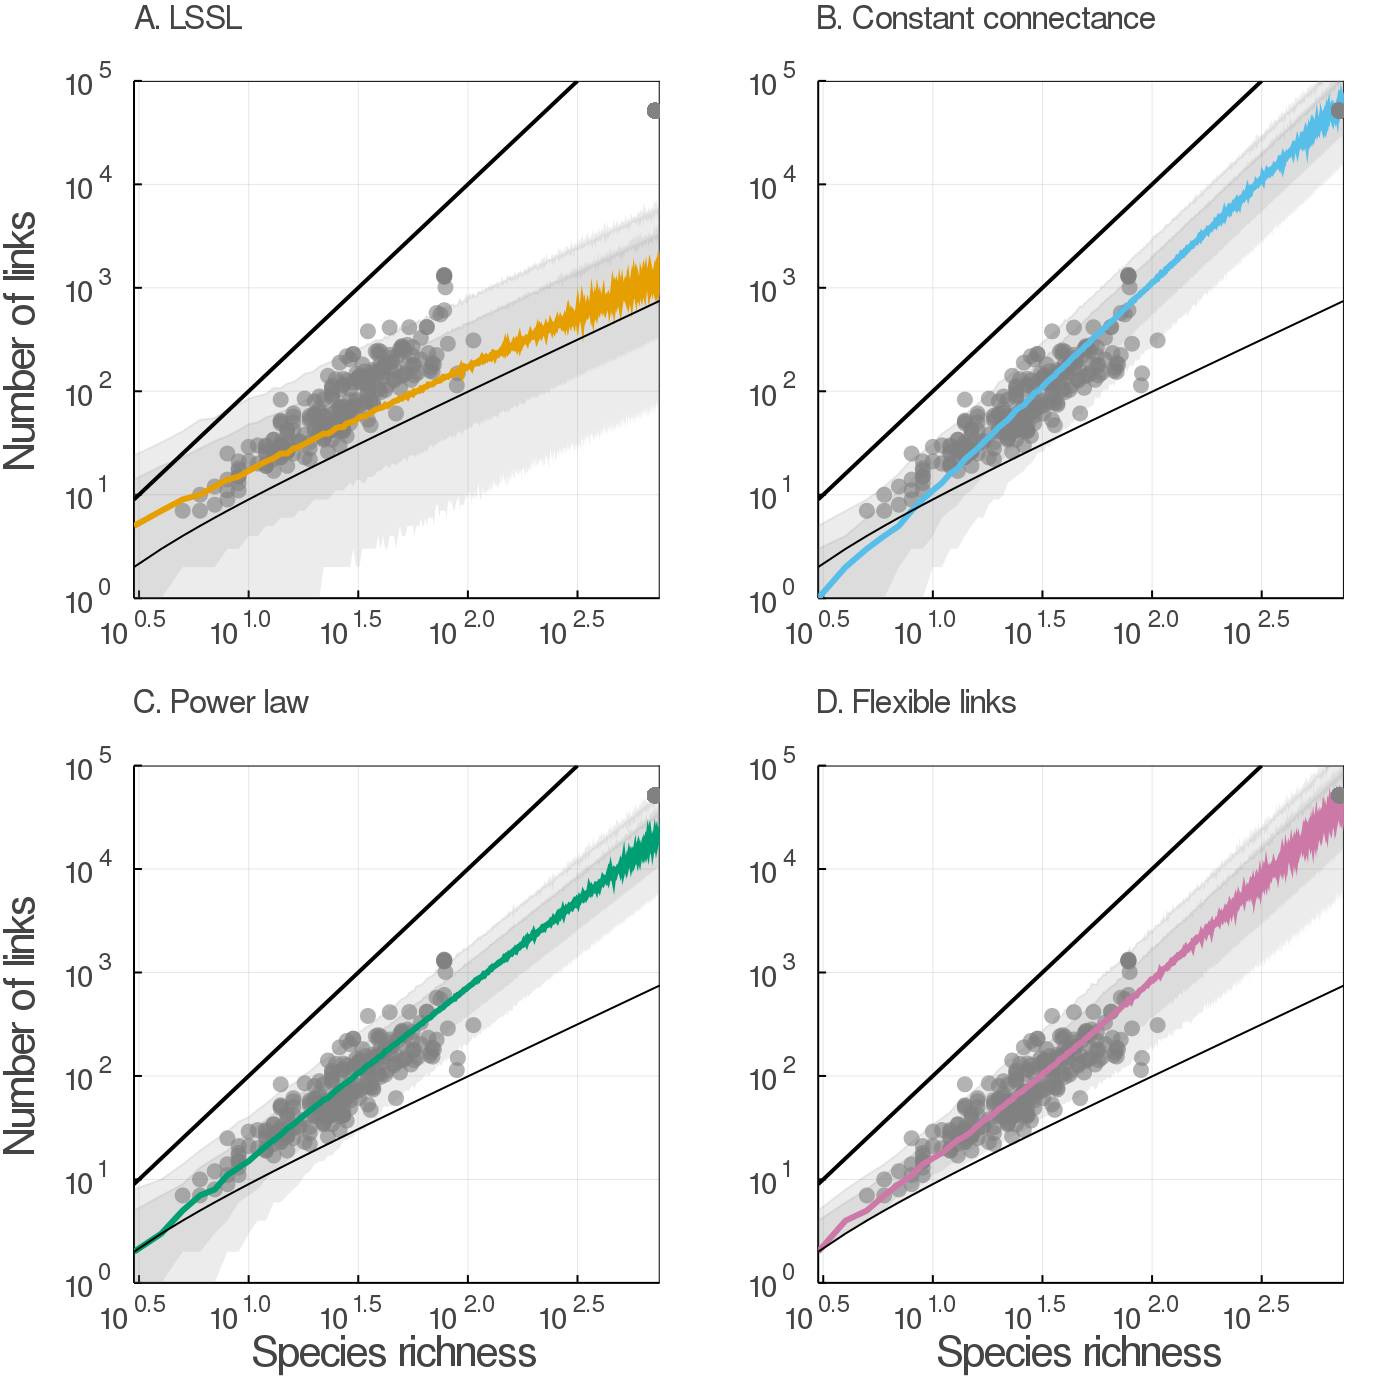
\includegraphics{figures/models_links.png}
\caption{\textbf{The flexible links model fits better and makes a
plausible range of predictions.} The number of links is plotted as a
function of species richness obtained from the posterior distributions
of A) the link-species scaling, B) the constant connectance, C) the
power law and D) the flexible links models. In each panel, the colored
line represents the median predicted link number and the grey areas
cover the 78\% and 97\% percentile intervals. Empirical data from the
\texttt{mangal.io} database are plotted in each panel (grey dots), as
well as the minimal \(S-1\) and maximal \(S^2\) number of links (thinner
and bolder black lines, respectively). Predictions from the flexible
links model are always plausible: they stay within these biological
boundaries.}\label{fig:PP_counterfactual}
}
\end{figure}

\hypertarget{the-flexible-links-model-makes-realistic-predictions-for-small-communities}{%
\subsection{The flexible links model makes realistic predictions for
small
communities}\label{the-flexible-links-model-makes-realistic-predictions-for-small-communities}}

Constraints on food web structure are especially important for small
communities. This is emphasized in \cref{fig:real_predict}, which shows
that all models other than the flexible links model fail to stay within
realistic ecological constraints when \(S\) is small. The link-species
scaling model made around 29\% of unrealistic predictions of link
numbers for every value of \(S\) (\(3 \leq S \leq 750\)). The constant
connectance and power law models, on the other hand, also produced
unrealistic results but for small networks only: more than 20\% were
unrealistic for networks comprising less than 12 and 7 species,
respectively. Only the flexible links model, by design, never failed to
predict numbers of links between \(S-1\) and \(S^2\). It must be noted
that unrealistic predictions are most common in the shaded area of
\cref{fig:real_predict}, which represents 90\% of the empirical data we
used to fit the model; therefore it matters little that models agree for
large \(S\), since there are virtually no such networks observed.

\begin{figure}
\hypertarget{fig:real_predict}{%
\centering
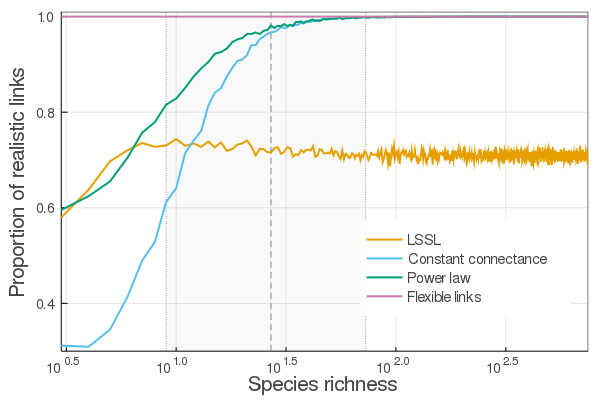
\includegraphics{figures/real_predict.png}
\caption{\textbf{Only the flexible links model makes realistic
predictions for small communities.} Here we show the proportion of
posterior predictions from each of our 4 models which fall outside
ecologically realistic values. The proportion of predictions in the
correct range increases with species richness for the constant
connectance and power law models. Shaded area shows the 5\%, 50\% and
95\% quantiles of the distribution of \(S\), demonstrating that many
communities have potentially incorrect predictions under previous
models.}\label{fig:real_predict}
}
\end{figure}

\hypertarget{parameter-estimates-for-all-models}{%
\subsection{Parameter estimates for all
models}\label{parameter-estimates-for-all-models}}

\begin{longtable}[]{@{}lllll@{}}
\caption{Parameter estimates for all models. Mean and standard deviation
(SD) are given for each parameter.
\label{tbl:parameters}}\tabularnewline
\toprule
Model & parameter & interpretation & value & SD\tabularnewline
\midrule
\endfirsthead
\toprule
Model & parameter & interpretation & value & SD\tabularnewline
\midrule
\endhead
\(bS\) {[}11{]} & \(b\) & links per species & 2.2 & 0.047\tabularnewline
& \(\kappa\) & concentration of \(L\) around mean & 1.4 &
0.12\tabularnewline
\(bS^2\) {[}12{]} & \(b\) & proportion of links realized & 0.12 &
0.0041\tabularnewline
& \(\kappa\) & concentration of \(L\) around mean & 4.0 &
0.37\tabularnewline
\(bS^a\) {[}13{]} & \(b\) & proportion of relationship & 0.37 &
0.054\tabularnewline
& \(a\) & scaling of relationship & 1.7 & 0.043\tabularnewline
& \(\kappa\) & concentration of \(L\) around mean & 4.8 &
0.41\tabularnewline
\((S^2 - (S - 1))p + S - 1\) & \(\mu\) & average value of \(p\) & 0.086
& 0.0037\tabularnewline
& \(\phi\) & concentration around value of \(\mu\) & 24.3 &
2.4\tabularnewline
\bottomrule
\end{longtable}

Although we did not use the same approach to parameter estimation as
previous authors, our approach to fitting these models recovered
parameter estimates that are broadly congruent with previous works. We
found a value of 2.2 for \(b\) of the LSSL model
(\cref{tbl:parameters}), which is close to the original value of
approximately 2 {[}11{]}. Similarly, we found a value of 0.12 for \(b\)
of the constant connectance model, which was consistent with original
estimates of 0.14 {[}12{]}. Finally, the parameter values we found for
the power law were also comparable to earlier estimates {[}13{]}. All of
these models were fit with a negative binomial observation model, which
has an additional parameter, \(\kappa\), which is sometimes called a
``concentration'' parameter. This value increases from the top of our
table to the bottom, in the same sequence as predictive performance
improves in \cref{tbl:comparison}. This indicates that the model
predictions are more concentrated around the mean predicted by the model
(\cref{tbl:parameters}, column 1).

Our parameter estimates for the flexible links model are ecologically
meaningful. For large communities, our model should behave similarly to
the constant connectance model and so it is no surprise that \(\mu\) was
about 0.09, which is close to our value of 0.12 for constant
connectance. In addition, we obtained a rather large value of 24.3 for
\(\phi\), which shrinks the variance around the mean of \(p\) to
approximately 0.003 (\(var(p)=\mu(1-\mu)/(1+\phi)\)). This indicates
that food webs are largely similar in their probability of flexible
links being realized (thus showing how our previous assumption that
\(p\) might vary between food webs to be more conservative than strictly
required). The flexible links model also uses fewer parameters than the
power law model and makes slightly better predictions, which accounts
for its superior performance in model comparison
(\cref{tbl:comparison}). In fig.~S1, we compare the maximum \emph{a
posteriori} (MAP) estimates of our model parameters to their maximum
likelihood estimates (MLE).

\hypertarget{connectance-and-linkage-density-can-be-derived-from-a-model-for-links}{%
\subsection{Connectance and linkage density can be derived from a model
for
links}\label{connectance-and-linkage-density-can-be-derived-from-a-model-for-links}}

Of the three important quantities which describe networks (\(L\), \(Co\)
and \(L_D\)), we have directly modelled \(L\) only. However, we can use
the parameter estimates from our model for \(L\) to parameterize a
distribution for connectance (\(L/S^2\)) and linkage density (\(L/S\)).
We can derive this by noticing that \cref{eq:lhat} can be rearranged to
show how \(Co\) and \(L_D\) are linear transformations of \(p\):

\begin{equation} Co = \frac{L}{S^2} = p\left(1 - \frac{S-1}{S^2}\right) + \frac{S-1}{S^2} ,\label{eq:co}\end{equation}

and

\begin{equation} L_D = \frac{L}{S} = p \left(S - \frac{S-1}{S} \right) +  \frac{S-1}{S},\label{eq:ld}\end{equation}

For food webs with many species, these equations simplify:
\cref{eq:lhat} can be expressed as a second degree polynomial,
\(L_{FL} = p\times S^2 + (1-p)\times S + (p-1)\), whose leading term is
\(p\times S^2\). Therefore, when \(S\) is large, \cref{eq:co} and
\cref{eq:ld} respectively approach \(Co = L/S^2 \approx p\) and
\(L_D = L/S \approx pS\). A study of \cref{eq:co} and \cref{eq:ld} also
provides insight into the ecological interpretation of the parameters in
our equation. For example, \cref{eq:ld} implies that adding \(n\)
species should increase the linkage density by approximately
\(p\times n\). The addition of 11 new species (\(p^{-1}\) according to
\cref{tbl:parameters}) should increase the linkage density in the food
web by roughly 1, meaning that each species in the original network
would be expected to develop 2 additional interactions. Similarly,
\cref{eq:co} shows that when \(S\) is large, we should expect a
connectance which is a constant. Thus \(p\) has an interesting
ecological interpretation: it represents the average connectance of
networks large enough that the proportion \((S-1)/S^{2}\) is negligible.

\hypertarget{applications-of-the-flexible-links-model-to-key-food-web-questions}{%
\subsection{Applications of the flexible links model to key food web
questions}\label{applications-of-the-flexible-links-model-to-key-food-web-questions}}

Our model is generative, and that is important and useful: we can use
this model to correctly generate predictions that look like real data.
This suggests that we can adapt the model, using either its parameters
or predictions or both, to get a new perspective on many questions in
network ecology. Here we show four possible applications that we think
are interesting, in that relying on our model eliminates the need to
speculate on the structure of networks, or to introduce new hypotheses
to account for it.

\hypertarget{probability-distributions-for-l_d-and-co}{%
\subsubsection{\texorpdfstring{Probability distributions for \(L_D\) and
\(Co\)}{Probability distributions for L\_D and Co}}\label{probability-distributions-for-l_d-and-co}}

In a beta-binomial distribution, it is assumed that the probability of
success \(p\) varies among groups of trials according to a
\(\text{Beta}(\mu\phi, (1-\mu)\phi)\) distribution. Since \(p\) has a
beta distribution, the linear transformations described by \cref{eq:co}
and \cref{eq:ld} also describe beta distributions which have been
shifted and scaled according to the number of species \(S\) in a
community. This shows that just as \(L\) must be within ecologically
meaningful bounds, \(Co\) (\cref{eq:co}) and \(L_D\) (\cref{eq:ld}) must
be as well. The connectance of a food web is bounded by \((S-1)/S^2\)
and \(1\), while the linkage density is bounded by \((S-1)/S\) and
\(S\).

We can convert the beta distribution for \(p\) into one for \(Co\) by
replacing \(p\) with the transformation of \(Co\) as described above
(\cref{eq:co}), and rescaling by the new range:

\begin{equation}
[Co | S, \mu, \phi] = \frac{\left(Co - \frac{S-1}{S^2}\right)^{\mu \phi - 1}\left(1 - Co\right)^{(1 - \mu)\phi - 1} }{\left(1 - \frac{S-1}{S^2}\right)^{\phi - 1} \times \mathrm{B}(\mu \phi, (1 - \mu)\phi)}
\label{eq:shiftBetaCo}\end{equation}

Similarly, we can convert the distribution for \(p\) into one for
\(L_D\) by replacing \(p\) with the transformation that gives \(L_D\)
(\cref{eq:ld})

\begin{equation}
[L_{D} | S, \mu, \phi] = \frac{\left(L_D - \frac{S-1} {S}\right)^{\mu \phi - 1}\left(1 - L_D\right)^{(1 - \mu)\phi - 1} }{\left(S - \frac{S-1}{S}\right)^{\phi - 1} \times \mathrm{B}(\mu \phi, (1 - \mu)\phi)}
\label{eq:shiftBetaLD}\end{equation}

In \cref{fig:CoLd}, we show that the connectance and linkage density
obtained from the equations above fit the empirical data well.

\begin{figure}
\hypertarget{fig:CoLd}{%
\centering
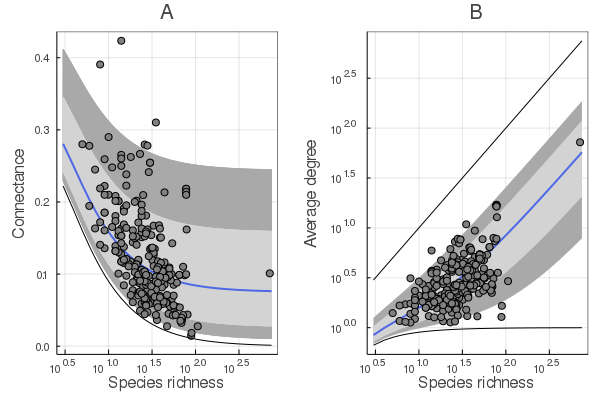
\includegraphics{figures/connectance_linkdens.png}
\caption{\textbf{Connectance and linkage density can be derived from a
model for links.} A) Connectance and B) linkage density are plotted as a
function of species richness, for the maximum \emph{a posteriori}
estimates of the flexible links model. In each panel, the colored line
represents the median predicted quantity and the grey areas cover the
78\% and 97\% percentile intervals. Empirical data from the
\texttt{mangal.io} database are plotted in each panel (grey dots). In
A), the minimal \((S-1)/S^2\) connectance and in B) the minimal
\((S-1)/S\) and maximum \(S\) linkage density are plotted (black
lines).}\label{fig:CoLd}
}
\end{figure}

\hypertarget{an-analytic-alternative-to-null-model-testing}{%
\subsubsection{An analytic alternative to null-model
testing}\label{an-analytic-alternative-to-null-model-testing}}

Ecologists are often faced with the issue of comparing several networks.
A common question is whether a given network has an ``unusual'' number
of links relative to some expectation. Traditionally these comparisons
have been done by simulating a ``null'' distribution of random matrices
{[}24,25{]}. This is intended to allow ecologists to compare food webs
to a sort of standard, hopefully devoid of whatever biological process
could alter the number of links. Importantly, this approach assumes that
(i) connectance is a fixed property of the network, ignoring any
stochasticity, and (ii) the simulated network distribution is an
accurate and unbiased description of the null distribution. Yet recent
advances in the study of probabilistic ecological networks show that the
existence of links, and connectance itself is best thought of as a
probabilistic quantity {[}18{]}. Given that connectance drives most of
the measures of food web structure {[}17{]}, it is critical to have a
reliable means of measuring differences from the expectation. We provide
a way to assess whether the number of links in a network (and therefore
its connectance) is surprising. We do so using maths rather than
simulations.

The shifted beta-binomial can be approximated by a normal distribution
with mean \(\bar{L}\) and variance \(\sigma_L^2\):

\[L \sim Normal(\bar{L}, \sigma_L^2)\]

\[\bar{L} = (S^2 - S + 1) \mu + S - 1\]

\begin{equation}\sigma_L^2 = (S^2 - S + 1) \mu (1 - \mu)(1 + \frac{S(S-1)}{\phi + 1})\label{eq:bb_sigma}\end{equation}

This normal approximation is considered good whenever the skewness of
the target distribution is modest. In food webs, this should be true
whenever communities have more than about 10 species (see Experimental
Procedures). This result means that given a network with observed
species richness \(S_{obs}\) and observed links \(L_{obs}\), we can
calculate its \(z\)-score, i.e.~how many standard deviations an
observation is from the population average, as

\begin{equation}z = \frac{L_{obs} - \bar{L}}{\sqrt{\sigma_L^2}} \,.\label{eq:z}\end{equation}

A network where \(L = \bar{L}\) will have a \(z\)-score of 0, and any
network with more (fewer) links will have a positive (negative)
\(z\)-score. Following this method, we computed the empirical
\(z\)-scores for the 255 food webs archived on \texttt{mangal.io}
(\cref{fig:zscores}). We found that 18 webs (7.1\%) had a total number
of observed links unusually higher than what was expected under the
flexible links model (\(z >\) 1.96). These networks are interesting
candidates for the study of mechanisms leading to high connectance.

Out of the 255 food webs, none was found to have an unusually low number
of links (\(z <\) 1.96). In fact, \(z\)-scores this low are not possible
in this dataset: food webs having the minimum value of \(S-1\) links are
still within two standard deviations of the mean, for this sample.
However, this sample contains the full diversity of food webs found in
the \texttt{mangal.io} database. Hence, this does not mean that no food
web will ever have a \(z\)-score lower than -1.96. If the flexible links
model is fit to data from a specific system, food webs might have a
surprisingly low number of links when compared to this population
average. These networks would be interesting candidates for the study of
mechanisms leading to low connectance or for the identification of
under-sampled webs. Ecologists can thus use our method to assess the
deviation of their own food webs from their random expectations.

\begin{figure}
\hypertarget{fig:zscores}{%
\centering
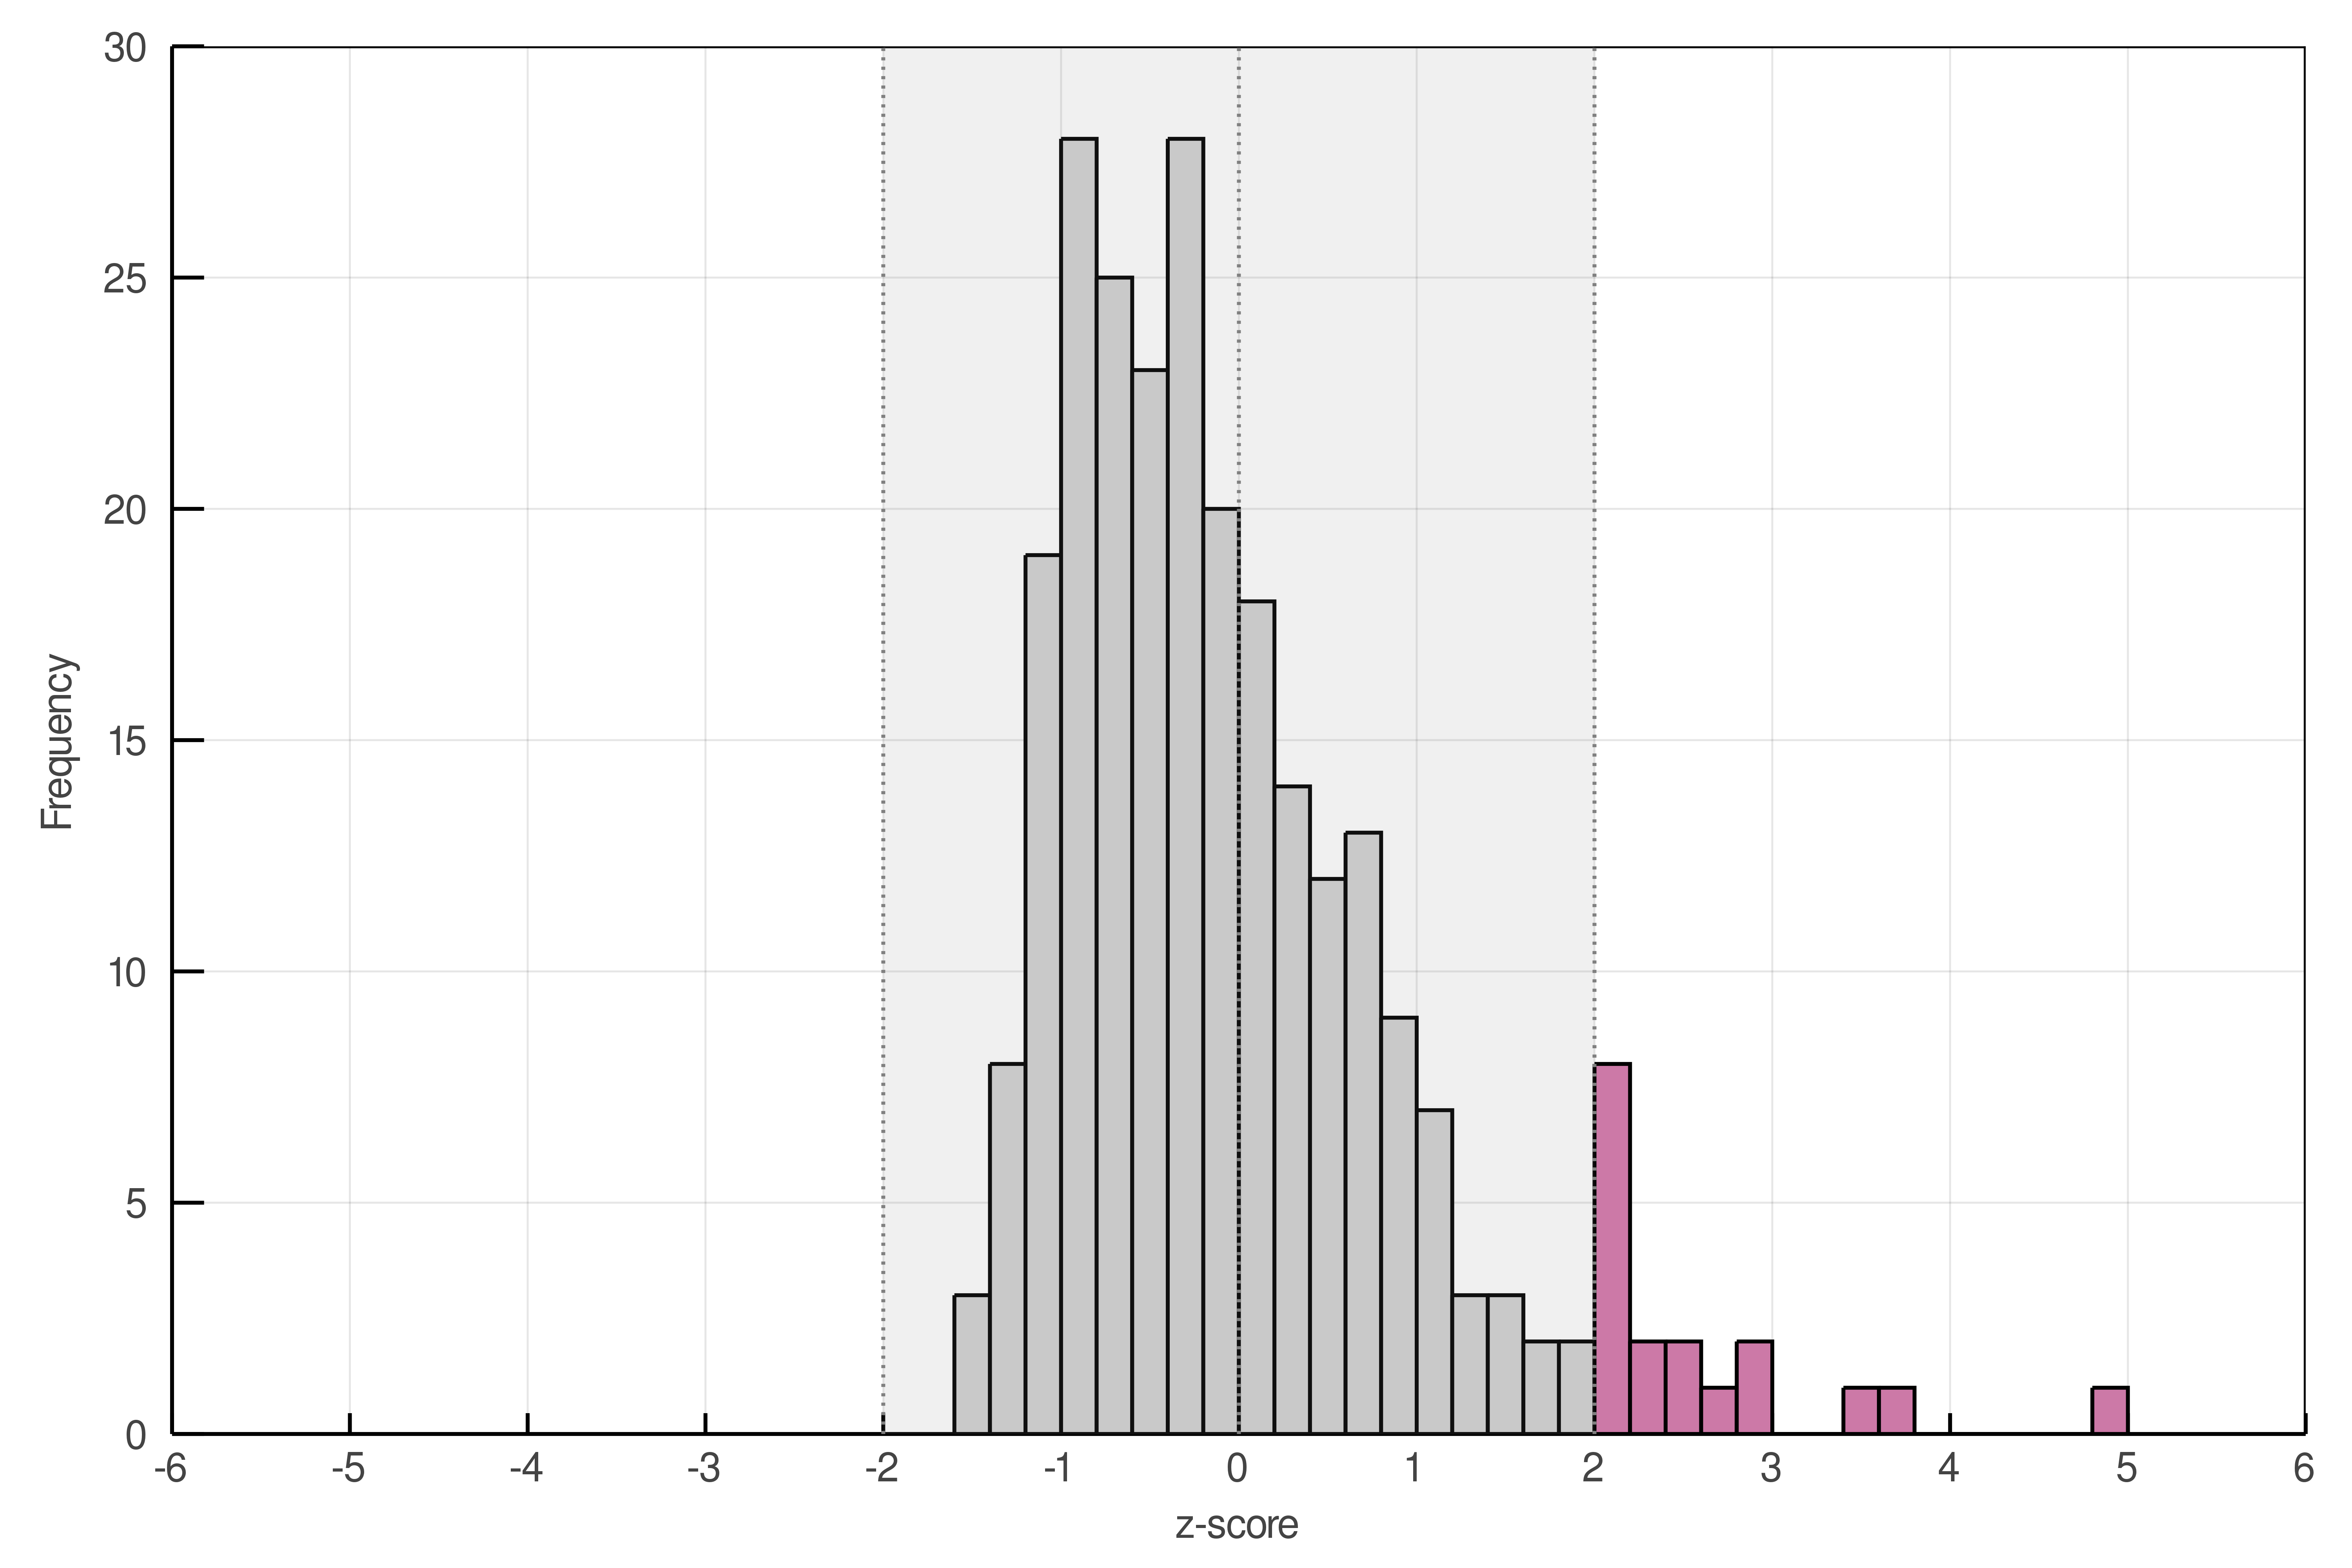
\includegraphics{figures/z-scores.png}
\caption{\textbf{Empirical distribution of food web \(z\)-scores} The
\(z\)-scores of all food webs archived on \texttt{mangal.io} have been
computed using \cref{eq:z}. Food webs with an absolute \(z\)-score above
1.96 are in pink. The shaded region comprises all food webs with an
absolute \(z\)-score below 1.96.}\label{fig:zscores}
}
\end{figure}

In \cref{fig:MAPnormal}, we show that the predictions made by the normal
approximation (panel B) are similar to those made by the beta
distribution parameterized with the maximum \emph{a posteriori} values
of \(\mu\) and \(\phi\) (panel A), although the former can undershoot
the constraint on the minimum number of links. This undershooting,
however, will not influence any actual \(z\)-scores, since no food webs
have fewer than \(S-1\) links and therefore no \(z\)-scores so low can
ever be observed.

\begin{figure}
\hypertarget{fig:MAPnormal}{%
\centering
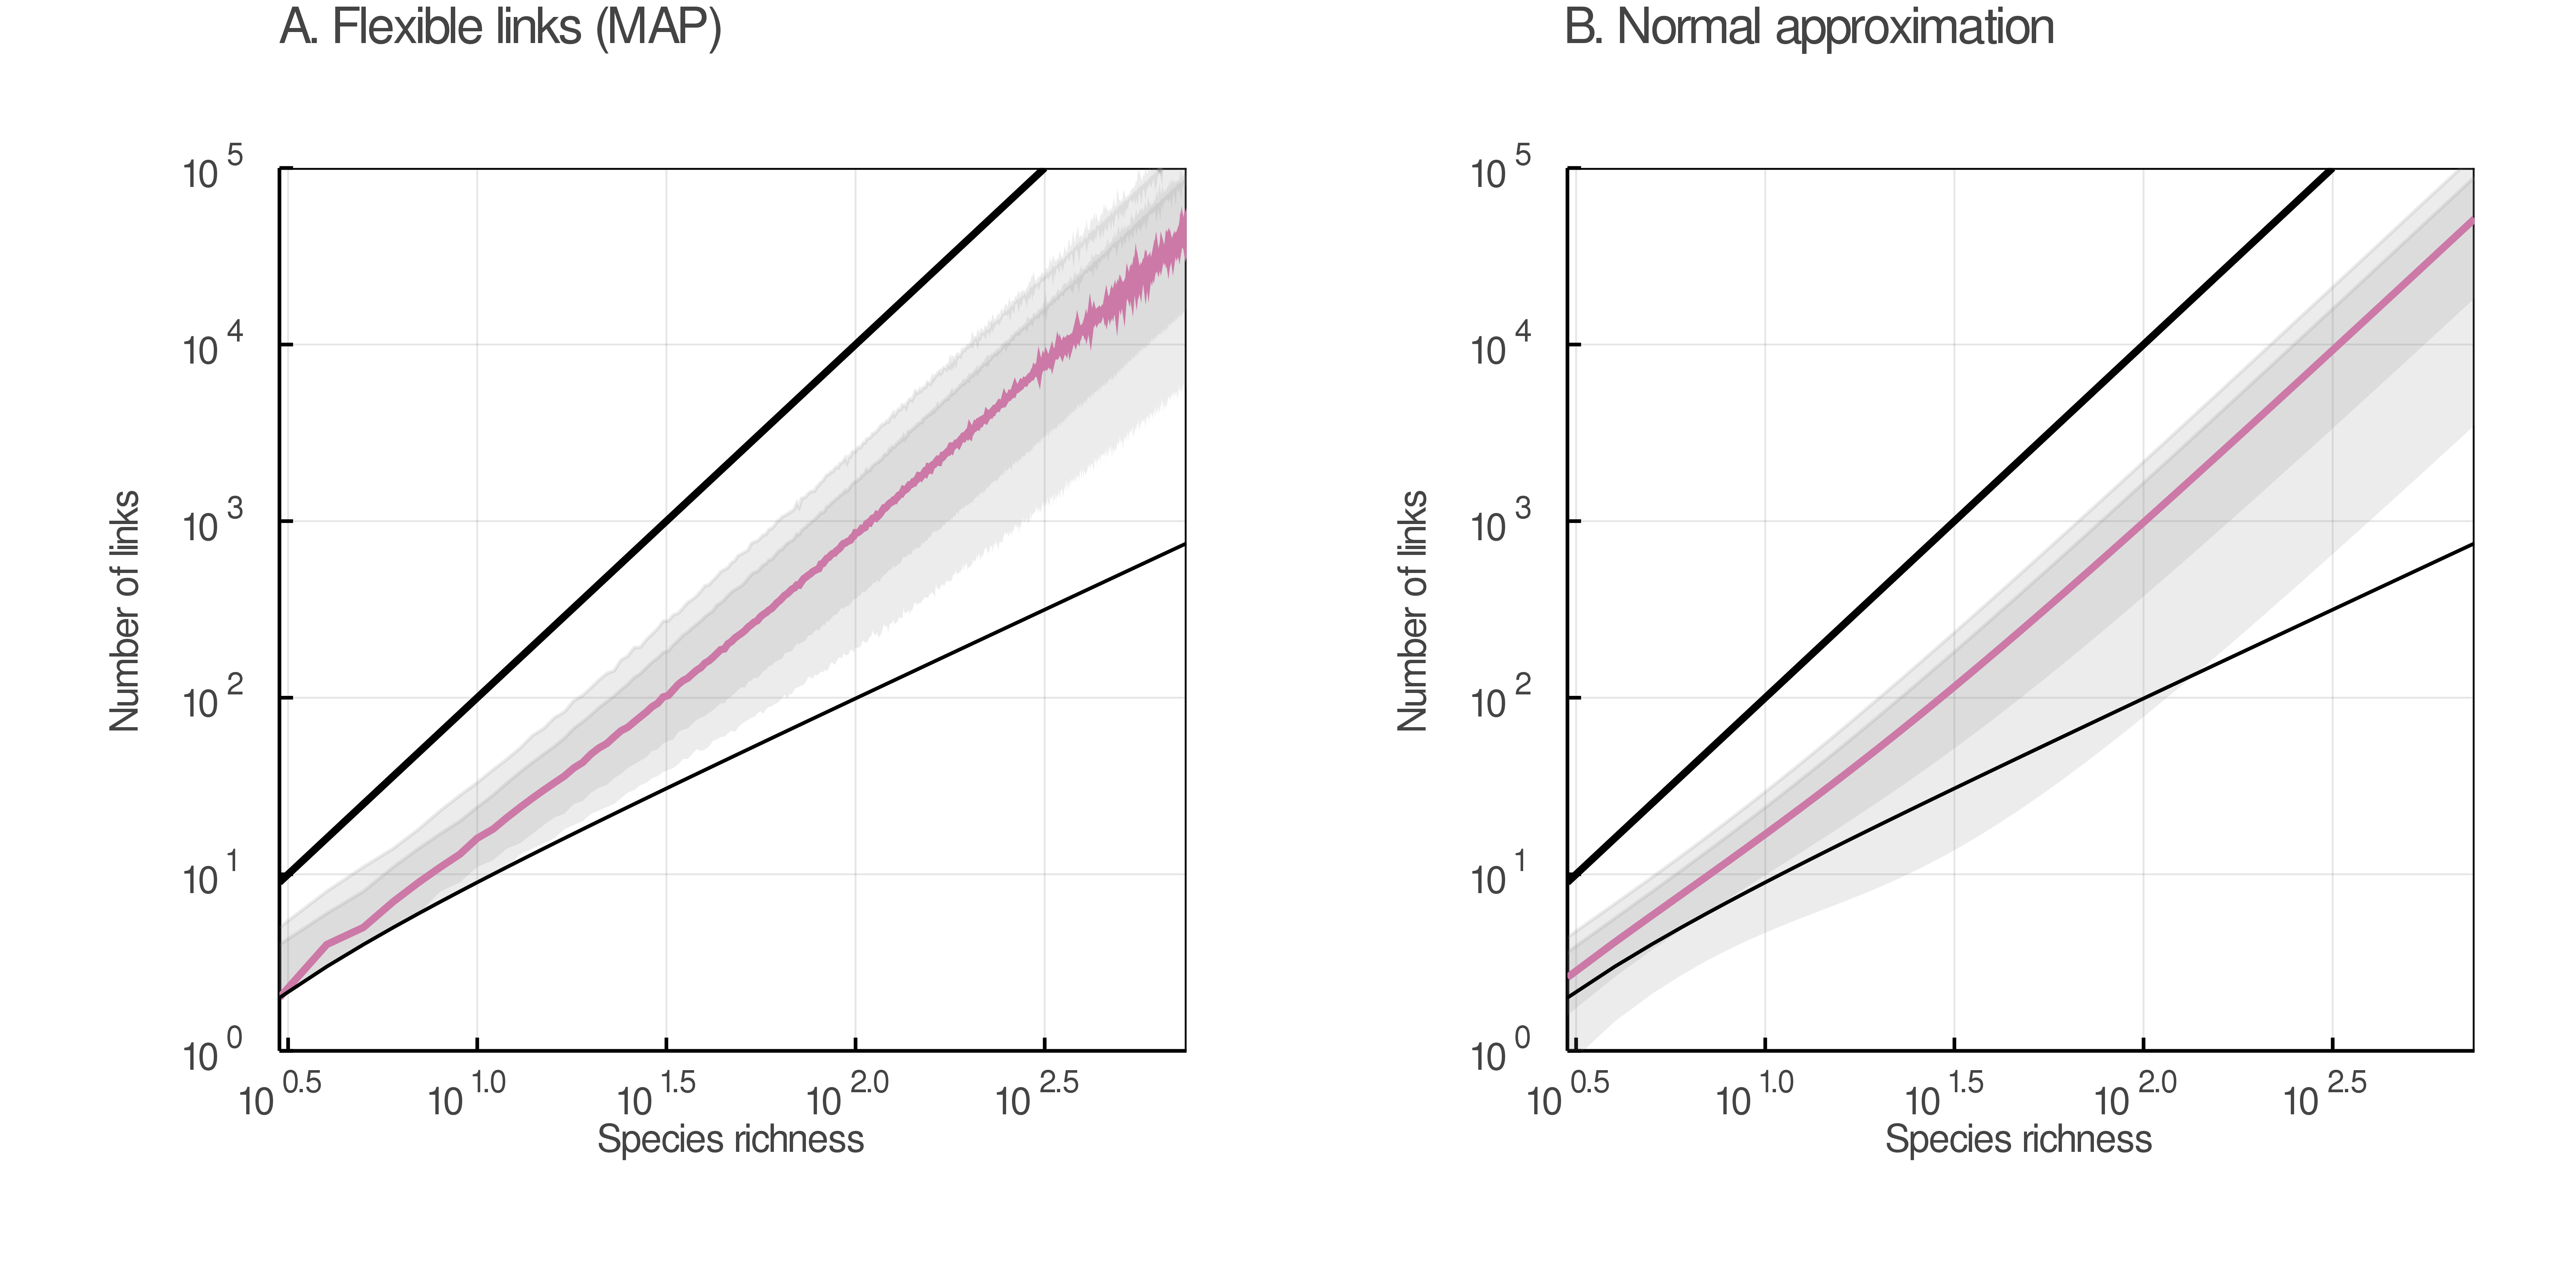
\includegraphics{figures/betabinmap_normal_links.png}
\caption{\textbf{The shifted beta-binomial distribution can be
approximated by a normal distribution.} The number of links is plotted
as a function of species richness obtained from A) the maximum \emph{a
posteriori} estimates of the flexible links model and B) its normal
approximation. In each panel, the colored line represents the median
predicted link number and the grey areas cover the 78\% and 97\%
percentile intervals. The minimal \(S-1\) and maximal \(S^2\) numbers of
links are plotted in each panel (thinner and bolder black lines,
respectively).}\label{fig:MAPnormal}
}
\end{figure}

\hypertarget{we-should-see-many-different-network-area-relationships}{%
\subsubsection{We should see many different network-area
relationships}\label{we-should-see-many-different-network-area-relationships}}

Our results bear important consequences for the nascent field of
studying network-area relationships {[}26{]}. As it has long been
observed that not all species in a food web diffuse equally through
space {[}27{]}, understanding how the shape of networks varies when the
area increases is an important goal, and in fact underpins the
development of a macroecological theory of food webs {[}28{]}. Using a
power-law as the acceptable relationship between species and area
{[}29,30{]}, the core idea of studying NAR is to predict network
structure as a consequence of the effect of spatial scale on species
richness {[}26{]}. Drawing on these results, we provide in
\cref{fig:nar} a simple illustration of the fact that, due to the
dispersal of values of \(L\), the relationship between \(L/S\) and area
can have a really wide confidence interval. While our posterior
predictions generally match the empirical results on this topic
{[}31{]}, they suggest that we will observe many relationships between
network structure and space, and that picking out the signal of
network-area relationships might be difficult.

As of now, not many NARs have been documented empirically; but after the
arguments made by {[}26{]} which tie the shape of these relationships to
macroecological processes, we fully expect these relationships to be
more frequently described moving forward. Our results suggest that our
expectation of the amount of noise in these relationships should be
realistic; while it is clear that these relationships exist, because of
the scaling of dispersion in the number of links with the number of
species, they will necessarily be noisy. Any described relationships
will exist within extremely wide confidence intervals, and it might
require a large quantity of empirical data to properly characterize
them. As such, our model can help in assessing the difficulty of
capturing some foundational relationships of food web structure.

\begin{figure}
\hypertarget{fig:nar}{%
\centering
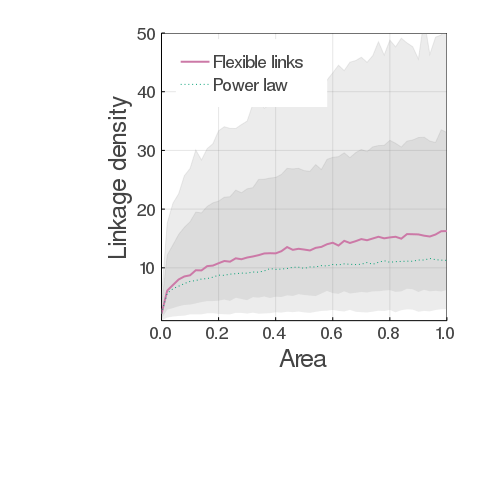
\includegraphics{figures/nar.png}
\caption{\textbf{Many different network-area relationships are supported
by the data}. Representing the species richness as \(S = k\times A^z\)
(panel A), with \(A\) being the relative area size, \(k = 200\) being
the maximal species richness, and \(z = 0.27\) a scaling exponent
{[}26{]}. We then use the posterior distribution of \(L\) to predict how
\(L_D\) should scale with \(A\). We compare the predictions of our model
to that of the generally accepted power law (\cref{eq:pl}). While our
model predicts a larger linkage density in larger areas (panel B), the
confidence intervals around this prediction (grey areas covering the
78\% and 97\% percentile intervals) are extremely large. In particular,
our model scales faster than the power law, but the confidence interval
is high (due to the scaling of variance with \(S\), \cref{eq:bb_sigma}).
This suggests that we may observe either very weak, or very strong,
effects of area on networks.}\label{fig:nar}
}
\end{figure}

\hypertarget{stability-imposes-a-limit-on-network-size}{%
\subsubsection{Stability imposes a limit on network
size}\label{stability-imposes-a-limit-on-network-size}}

Can organisms really interact with an infinite number of partners?
According to \cref{eq:ld}, at large values of \(S\), the linkage density
scales according to \(p\times S\) (which is supported by empirical
data), and so species are expected to have on average
\(2\times p\times S\) interactions. A useful concept in evolutionary
biology is the ``Darwinian demon'' {[}32{]}, \emph{i.e.} an organism
that would have infinite fitness in infinite environments. Our model
seems to predict the emergence of what we call Eltonian demons, which
can have arbitrarily large number of interactions. Yet we know that
constraints on handling time of prey, for example, imposes hard limits
on diet breadth {[}33{]}. This result suggests that there are other
limitations to the size of food webs; indeed, the fact that \(L/S\)
increases to worryingly large values only matters if ecological
processes allow \(S\) to be large enough. It is known that food webs can
get as high as energy transfer allows {[}5{]}, and as wide as
competition allows {[}34{]}. Furthermore, in more species-rich
communities there is a greater diversity of functional traits among the
interacting organisms; this limits interactions, because traits
determine suitable interaction partners {[}35,36{]}. In short, and as
\cref{fig:real_predict} suggests, since food webs are likely to be
constrained to remain within an acceptable richness, we have no reason
to anticipate that \(p\times S\) will keep growing infinitely.

Network structure may itself prevent \(S\) from becoming large. May
{[}37{]} suggested that a network of richness \(S\) and connectance
\(Co\) is stable as long as the criteria
\(\sigma \sqrt{S \times Co} < 1\) is satisfied, with \(\sigma\) being
the standard deviation of the strengths of interactions. Although this
criteria is not necessarily stringent enough for the stability of food
webs {[}38,39{]}, it still defines an approximate maximum value
\(\sigma^\star\) which is the value above which the system is expected
to be unstable. This threshold is \(\sigma^\star = 1/\sqrt{L_D}\), where
\(L_D\) is defined as in \cref{eq:ld}. We illustrate this result in
\cref{fig:stability}, which reveals that \(\sigma^\star\) falls towards
0 for larger species richness. The result in \cref{fig:stability} is in
agreement with previous simulations, placing the threshold for stability
at about 1200 species in food webs. These results show how ecological
limitations, for example on connectance and the resulting stability of
the system, can limit the size of food webs {[}38,40{]}. In the second
panel, we show that networks of increasing richness (thicker lines,
varying on a log-scale from \(10^1\) to \(10^3\)) have a lower
probability of being stable, based on the proportion of stable networks
in our posterior samples.

\begin{figure}
\hypertarget{fig:stability}{%
\centering
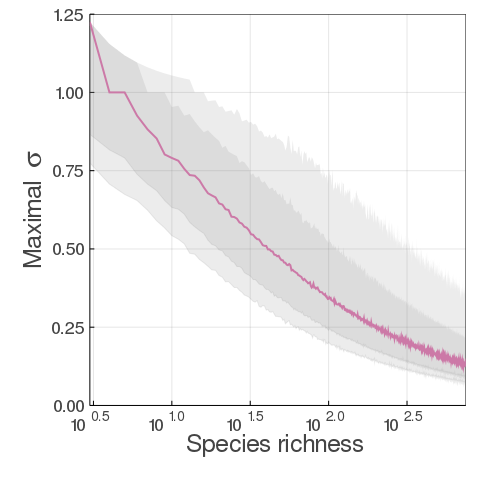
\includegraphics{figures/may.png}
\caption{\textbf{Stability imposes a limit on network size}. Using
\cref{eq:ld}, we can calculate the maximum standard deviation in the
strength of interactions which should ensure food web stability,
\(\sigma^\star = 1/\sqrt{L_D}\) (panel A). The colored line represent
the median value of maximum standard deviation, based on the posterior
distribution of the flexible links model, and the grey areas cover the
78\% and 97\% percentile intervals. The fine and dark lines indicate the
maximum and minimum values of maximum standard deviation, respectively.
The dotted line shows the maximum for the average \(L_D\), as given by
\cref{eq:ld}. The maximum standard deviation falls sharply when the
number of species increases, which will limit the stability of large
food webs, and therefore explain why Eltonian demons should not emerge.
In panel B, we show the probability of a network with \(S\) species
being stable, based on draws from the posterior distribution, for
\(10 \le S \le 1000\) - larger networks (thicker lines) are increasingly
unlikely to be stable.}\label{fig:stability}
}
\end{figure}

\hypertarget{conclusions}{%
\subsection{Conclusions}\label{conclusions}}

Here we derived \cref{eq:lhat}, a model for the prediction of the number
of links in ecological networks using a beta-binomial distribution for
\(L\), and show how it outperforms previous and more commonly used
models describing this relationship. More importantly, we showed that
our model has parameters with a clear ecological interpretation
(specifically, the value of \(p\) in \cref{eq:lhat} is the expected
value of the connectance when \(S\) is large), and makes predictions
which remain within biological boundaries. There are a variety of
``structural'' models for food webs, such as the niche model {[}41{]},
the cascade model {[}42{]}, the DBM {[}35{]} and ADBM {[}19{]}, the
minimum potential niche model {[}43{]}, and the nested hierarchy model
{[}44{]} to name a few. All of these models make predictions of food web
structure: based on some parameters (usually \(S\) and \(L\), and
sometimes vectors of species-level parameters) they output an adjacency
matrix \(\mathbf{A}_{S\times S}\) which contains either the presence or
strength of trophic interactions. Therefore, these models require
estimated values of \(L\) for a particular value of \(S\), with the
additional result that \(\sum \mathbf{A} = L\). Our approach can serve
to improve the realism of these models, by imposing that the values of
\(L\) they use are within realistic boundaries. For example, a common
use of structural models is to generate a set of ``null'' predictions:
possible values of \(\mathbf{A}\) and \(L\) in the absence of the
mechanism of interest. Empirical networks are then compared to this set
of predictions, and are said to be significant if they are more extreme
than 95\% of the observations {[}3{]}. A challenge in this approach is
that structural models may generate a wide range of predictions,
including ecologically impossible values, leading a high false negative
rate. This could be remedied by filtering this set of predictions
according to our flexible links model, resulting in a narrower set of
null predictions and a lower false negative rate. In general, our
approach is complementary to other attempts to create
ecologically-realistic food web models; for example, probabilistic
models of the number of links per species which stay within ecological
values {[}45{]}.

This model also casts new light on previous results on the structure of
food webs: small and large food webs behave differently {[}15{]}.
Specifically, ecological networks most strongly deviate from scale free
expectations when connectance is high {[}46{]}. In our model, this
behaviour emerges naturally: connectance increases sharply as species
richness decreases (\cref{fig:CoLd}) -- that is, where the additive term
\((S-1)/S^{2}\) in \cref{eq:co} becomes progressively larger. In a
sense, small ecological networks are different only due to the low
values of \(S\). Small networks have only a very limited number of
flexible links, and this drives connectance to be greater. Connectance
in turn has implications for many ecological properties. Connectance is
more than the proportion of realized interactions. It has been
associated with some of the most commonly used network measures
{[}17{]}, and contains meaningful information on the stability
{[}46,47{]} and dynamics {[}48{]} of ecological communities. A
probability distribution for connectance not only accounts for the
variability between networks, but can be used to describe fundamental
properties of food webs and to identify ecological and evolutionary
mechanisms shaping communities. A recent research direction has been to
reveal its impact on resistance to invasion: denser networks with a
higher connectance are comparatively more difficult to invade {[}49{]};
different levels of connectance are also associated with different
combinations of primary producers, consumers, and apex predators
{[}41{]}, which in turns determines which kind of species will have more
success invading the network {[}50{]}. Because we can infer connectance
from the richness of a community, our model also ties the invasion
resistance of a network to its species richness.

The relationship between \(L\) and \(S\) has underpinned most of the
literature on food web structure since the 1980s. Additional generations
of data have allowed us to progress from the link-species scaling law,
to constant connectance, to more general formulations based on a power
law. Our model breaks with this tradition of iterating over the same
family of relationships, and instead draws from our knowledge of
ecological processes, and from novel tools in probabilistic programming.
As a result, we provide predictions of the number of links which are
closer to empirical data, stimulate new ecological insights, and can be
safely assumed to always fall within realistic values. The results
presented in \cref{fig:nar} (which reproduces results from {[}26{]}) and
\cref{fig:stability} (which reproduces results from {[}38{]}) may seem
largely confirmatory; in fact, the ability of our model to reach the
conclusions of previous milestone studies in food web ecology is a
strong confirmation of its validity. We would like to point out that
these approaches would usually require ecologists to make inferences not
only on the parameters of interests, but also on the properties of a
network for a given species richness. In contrast, our model allows a
real economy of parameters and offers ecologists the ability to get
several key elements of network structure for free if only the species
richness is known.

\hypertarget{experimental-procedures}{%
\section{Experimental Procedures}\label{experimental-procedures}}

\hypertarget{availability-of-code-and-data}{%
\subsubsection{Availability of code and
data}\label{availability-of-code-and-data}}

All code and data to reproduce this article is available at the Open
Science Framework (DOI:
\href{https://doi.org/10.17605/OSF.IO/YGPZ2}{10.17605/OSF.IO/YGPZ2}).

\hypertarget{bayesian-model-definitions}{%
\subsubsection{Bayesian model
definitions}\label{bayesian-model-definitions}}

Generative models are flexible and powerful tools for understanding and
predicting natural phenomena. These models aim to create simulated data
with the same properties as observations. Creating such a model involves
two key components: a mathematical expression which represents the
ecological process being studied, and a distribution which represents
our observations of this process. Both of these components can capture
our ecological understanding of a system, including any constraints on
the quantities studied.

Bayesian models are a common set of generative models, frequently used
to study ecological systems. Here, we define Bayesian models for all 4
of the models described in \cref{eq:lssl}, \cref{eq:cc}, \cref{eq:pl}
and \cref{eq:lhat}. We use notation from {[}51{]}, writing out both the
likelihood and the prior as a product over all 255 food webs in the
\texttt{mangal.io} database.

Link-species scaling (LSSL) model:

\[
[b, \kappa | \textbf{L}, \textbf{S}] \propto \prod_{i = 1}^{255} \text{negative binomial}(L_i | b \times S_i, e^{\kappa}) \times \text{normal}(b|0.7, 0.02) \times \text{normal}(\kappa|2, 1)
\]

Constant connectance model:

\[
[b, \kappa | \textbf{L}, \textbf{S}] \propto \prod_{i = 1}^{255} \text{negative binomial}(L_i | b \times S_i^2, e^{\kappa}) \times \text{beta}(b|3, 7) \times \text{normal}(\kappa|2, 1)
\]

Power law model:

\[
[b, a, \kappa | \textbf{L}, \textbf{S}] \propto \prod_{i = 1}^{255} \text{negative binomial}(L_i | \exp(b) \times S_i^a, e^{\kappa}) \times \text{normal}(b| -3 , 1) \times \text{normal}(a | 2, 0.6) \times \text{normal}(\kappa|2, 1)
\]

Flexible links model:

\[
[\mu, \phi| \textbf{L}, \textbf{S}] \propto \prod_{i = 1}^{255} \text{beta binomial}(L_i - S_i + 1 | S_i^2 - S_i + 1, \mu \times e^{\phi}, (1 - \mu) \times e^\phi) \times \text{beta}(\mu| 3 , 7 ) \times \text{normal}(\phi | 3, 0.5)
\]

Note that while \(e^\phi\) is shown in these equations for clarity, in
the text we use \(\phi\) to refer to the parameter after exponentiation.
In the above equations, bold type indicates a \emph{vector} of values;
we use capital letters for \(\textbf{L}\) and \(\textbf{S}\) for
consistency with the main text.

Because we want to compare all our models using information criteria, we
were required to use a discrete likelihood to fit all models. Our model
uses a discrete likelihood by default, but the previous three models
(LSSL, constant connectance and the power law) normally do not. Instead,
these models have typically been fit with Gaussian likelihoods,
sometimes after log-transforming \(L\) and \(S\). For example,
\cref{eq:pl} becomes a linear relationship between \(\text{log}(L)\) and
\(\text{log}(S)\). This ensures that predictions of \(L\) are always
positive, but allows otherwise unconstrained variation on both sides of
the mean. To keep this same spirit, we chose the negative binomial
distribution for observations. This distribution is limited to positive
integers, and can vary on both sides of the mean relationship.

We selected priors for our Bayesian models using a combination of
literature and domain expertise. For example, we chose our prior
distribution for \(p\) based on {[}12{]} , who gave a value of constant
connectance equal to 0.14. While the prior we use is ``informative'', it
is weakly so; as {[}12{]} did not provide an estimate of the variance
for his value we chose a relatively large variation around that mean.
However, no information is available in the literature to inform a
choice of prior for concentration parameters \(\kappa\) and \(\phi\).
For these values, we followed the advice of {[}52{]} and performed prior
predictive checks. Specifically, we chose priors that generated a wide
range of values for \(L_i\), but which did not frequently predict webs
of either maximum or minimum connectance, neither of which are observed
in nature.

\hypertarget{explanation-of-shifted-beta-binomial-distribution}{%
\subsubsection{Explanation of shifted beta-binomial
distribution}\label{explanation-of-shifted-beta-binomial-distribution}}

Equation \cref{eq:lhat} implies that \(L_{FL}\) has a binomial
distribution, with \(S^2 - S + 1\) trials and a probability \(p\) of any
flexible link being realized:

\[
[L | S, p] = { S^2 - (S - 1) \choose L - (S - 1)} p^{L-(S-1)}(1-p)^{S^2 - L} ,
\]

This is often termed a \emph{shifted binomial distribution}.

We also note that ecological communities are different in many ways
besides their number of species (\(S\)). Although we assume \(p\) to be
fixed within one community, the precise value of \(p\) will change from
one community to another. With this assumption, our likelihood becomes a
shifted beta-binomial distribution:

\begin{equation}
[L|S,\mu, \phi] =  { S^2 - (S - 1) \choose L - (S - 1)} \frac{\mathrm{B}(L - (S - 1) + \mu \phi, S^2 - L + (1 - \mu)\phi)}{\mathrm{B}(\mu \phi, (1 - \mu)\phi)}
\label{eq:shiftBB2}\end{equation}

Where \(B\) is the beta function. Thus, the problem of fitting this
model becomes one of estimating the parameters of this univariate
probability distribution.

\hypertarget{model-fitting---data-and-software}{%
\subsection{Model fitting - data and
software}\label{model-fitting---data-and-software}}

We evaluated our model against 255 empirical food webs, available in the
online database \texttt{mangal.io} {[}21{]}. We queried metadata (number
of nodes and number of links) for all networks, and considered as food
webs all networks having interactions of predation and herbivory. We use
Stan {[}53{]} which implements Bayesian inference using Hamiltonian
Monte Carlo. We ran all models using four chains and 2000 iterations per
chain. In our figures we use the posterior predictive distribution,
which is a distribution described by the model after conditioning on the
data. There are numerous ways to display a probability distribution;
here we have chosen to do so using the expectation (mean) and two
arbitrary percentile intervals: 78\% and 97\%. These intervals were
chosen based on the recommendations of {[}54{]}, and allowed us to
capture most of the probability density in the tails of the posterior
distributions.

Stan provides a number of diagnostics for samples from the posterior
distribution, including \(\hat{R}\), effective sample size, and measures
of effective tree depth and divergent iterations. None of these
indicated problems with the posterior sampling. All models converged
with no warnings; this indicates that is it safe to make inferences
about the parameter estimates and to compare the models. However, the
calculation of PSIS-LOO for the LSSL model warned of problematic values
of the Pareto-k diagnostic statistic. This indicates that the model is
heavily influenced by large values. Additionally, we had to drop the
largest observation (\textgreater{} 50 000 links) from all datasets in
order to calculate PSIS-LOO for the LSSL model. Taken together, this
suggests that the LSSL model is insufficiently flexible to accurately
reproduce the data.

\hypertarget{normal-approximation-and-analytic-z-scores}{%
\subsection{\texorpdfstring{Normal approximation and analytic
\(z\)-scores}{Normal approximation and analytic z-scores}}\label{normal-approximation-and-analytic-z-scores}}

We propose using a normal approximation to the beta-binomial
distribution, to calculate analytic \(z\)-scores. This is based on a
well-known similarity between the shape of a normal distribution and a
binomial distribution. This approximation is considered good whenever
the absolute skewness is less than 0.3 {[}55{]}, that is whenever:

\[
\frac{1}{\sqrt{S^2 - S + 1}}\left(\sqrt{\frac{1- \mu}{\mu}} - \sqrt{\frac{\mu}{1-\mu}}\right) < 0.3
\]

The beta-binomial distribution is close to the binomial distribution.
The error in approximating the former with the latter is on the order of
the inverse square of the parameter \(\phi\) {[}56{]}, which for our
model is less than 0.0017.

\hypertarget{acknowledgments}{%
\section{Acknowledgments}\label{acknowledgments}}

We thank three anonymous reviewers, as well as Owen Petchey and Andrew
Beckerman, for their helpful comments and suggestions. Funding was
provided by the Institute for data valorization (IVADO) and the NSERC
CREATE Computational Biodiversity Science and Services (BIOS\(^2\))
training program. TP acknowledges funding from the John Evans Leaders'
funds from the Canadian Foundation for Innovation. This work was made
possible thanks to the effort of volunteers developing high-quality free
and open source software for research.

\hypertarget{references}{%
\section*{References}\label{references}}
\addcontentsline{toc}{section}{References}

\hypertarget{refs}{}
\begin{cslreferences}
\leavevmode\hypertarget{ref-BorrMood14}{}%
1. Borrett, S.R., Moody, J., and Edelmann, A. (2014). The rise of
Network Ecology: Maps of the topic diversity and scientific
collaboration. Ecological Modelling \emph{293}, 111--127.

\leavevmode\hypertarget{ref-cana12esp}{}%
2. Canard, E., Mouquet, N., Marescot, L., Gaston, K.J., Gravel, D., and
Mouillot, D. (2012). Emergence of Structural Patterns in Neutral Trophic
Networks. PLOS ONE \emph{7}, e38295. Available at:
\url{http://journals.plos.org/plosone/article?id=10.1371/journal.pone.0038295}.

\leavevmode\hypertarget{ref-DelmBess18}{}%
3. Delmas, E., Besson, M., Brice, M.-H., Burkle, L.A., Dalla Riva, G.V.,
Fortin, M.-J., Gravel, D., Guimarães, P.R., Hembry, D.H., and Newman,
E.A. \emph{et al.} (2018). Analysing ecological networks of species
interactions. Biological Reviews, 112540. Available at:
\url{http://doi.wiley.com/10.1111/brv.12433}.

\leavevmode\hypertarget{ref-McCa12}{}%
4. McCann, K.S. (2012). Food webs (Princeton: Princeton University
Press).

\leavevmode\hypertarget{ref-ThomBros12}{}%
5. Thompson, R.M., Brose, U., Dunne, J.A., Hall, R.O., Hladyz, S.,
Kitching, R.L., Martinez, N.D., Rantala, H., Romanuk, T.N., and
Stouffer, D.B. \emph{et al.} (2012). Food webs: reconciling the
structure and function of biodiversity. Trends in Ecology \& Evolution
\emph{27}, 689--697.

\leavevmode\hypertarget{ref-McCa07}{}%
6. McCann, K. (2007). Protecting biostructure. Nature \emph{446},
29--29. Available at:
\url{http://www.nature.com/nature/journal/v446/n7131/full/446029a.html}.

\leavevmode\hypertarget{ref-SeibCado18}{}%
7. Seibold, S., Cadotte, M.W., MacIvor, J.S., Thorn, S., and Müller, J.
(2018). The Necessity of Multitrophic Approaches in Community Ecology.
Trends in Ecology \& Evolution \emph{33}, 754--764. Available at:
\url{https://www.cell.com/trends/ecology-evolution/abstract/S0169-5347(18)30147-2}.

\leavevmode\hypertarget{ref-Jord16a}{}%
8. Jordano, P. (2016). Sampling networks of ecological interactions.
Functional Ecology \emph{30}, 1883--1893. Available at:
\url{http://doi.wiley.com/10.1111/1365-2435.12763}.

\leavevmode\hypertarget{ref-Jord16}{}%
9. Jordano, P. (2016). Chasing Ecological Interactions. PLOS Biol
\emph{14}, e1002559. Available at:
\url{http://journals.plos.org/plosbiology/article?id=10.1371/journal.pbio.1002559}.

\leavevmode\hypertarget{ref-PascDunn06}{}%
10. Pascual, M., and Dunne, J.A. (2006). Ecological Networks: Linking
Structure to Dynamics in Food Webs (Oxford University Press, USA).

\leavevmode\hypertarget{ref-CoheBria84}{}%
11. Cohen, J.E., and Briand, F. (1984). Trophic links of community food
webs. Proc Natl Acad Sci U S A \emph{81}, 4105--4109.

\leavevmode\hypertarget{ref-mart92ccc}{}%
12. Martinez, N.D. (1992). Constant Connectance in Community Food Webs.
The American Naturalist \emph{139}, 1208--1218. Available at:
\url{http://www.jstor.org/stable/2462337}.

\leavevmode\hypertarget{ref-BrosOstl04}{}%
13. Brose, U., Ostling, A., Harrison, K., and Martinez, N.D. (2004).
Unified spatial scaling of species and their trophic interactions.
Nature \emph{428}, 167--171. Available at:
\url{http://dx.doi.org/10.1038/nature02297}.

\leavevmode\hypertarget{ref-WinePian01}{}%
14. Winemiller, K., Pianka, E., Vitt, L., and Joern, A. (2001). Food Web
Laws or Niche Theory? Six Independent Empirical Tests. The American
Naturalist \emph{158}, 193--199. Available at:
\url{https://www.journals.uchicago.edu/doi/abs/10.1086/321315}.

\leavevmode\hypertarget{ref-GarlCald03}{}%
15. Garlaschelli, D., Caldarelli, G., and Pietronero, L. (2003).
Universal scaling relations in food webs. Nature \emph{423}, 165--168.
Available at: \url{https://www.nature.com/articles/nature01604}.

\leavevmode\hypertarget{ref-RiedRall10}{}%
16. Riede, J.O., Rall, B.C., Banasek-Richter, C., Navarrete, S.A.,
Wieters, E.A., Emmerson, M.C., Jacob, U., and Brose, U. (2010). Chapter
3 - Scaling of Food-Web Properties with Diversity and Complexity Across
Ecosystems. In Advances in Ecological Research Ecological Networks., G.
Woodward, ed. (Academic Press), pp. 139--170. Available at:
\url{http://www.sciencedirect.com/science/article/pii/B9780123813633000034}.

\leavevmode\hypertarget{ref-PoisGrav14}{}%
17. Poisot, T., and Gravel, D. (2014). When is an ecological network
complex? Connectance drives degree distribution and emerging network
properties. PeerJ \emph{2}, e251. Available at:
\url{https://peerj.com/articles/251}.

\leavevmode\hypertarget{ref-PoisCirt16}{}%
18. Poisot, T., Cirtwill, A.R., Cazelles, K., Gravel, D., Fortin, M.-J.,
and Stouffer, D.B. (2016). The structure of probabilistic networks.
Methods in Ecology and Evolution \emph{7}, 303--312. Available at:
\url{http://doi.wiley.com/10.1111/2041-210X.12468}.

\leavevmode\hypertarget{ref-PetcBeck08}{}%
19. Petchey, O.L., Beckerman, A.P., Riede, J.O., and Warren, P.H.
(2008). Size, foraging, and food web structure. Proceedings of the
National Academy of Sciences \emph{105}, 4191--4196. Available at:
\url{http://www.pnas.org/cgi/doi/10.1073/pnas.0710672105}.

\leavevmode\hypertarget{ref-PoisStou15}{}%
20. Poisot, T., Stouffer, D.B., and Gravel, D. (2015). Beyond species:
why ecological interaction networks vary through space and time. Oikos
\emph{124}, 243--251. Available at:
\url{http://doi.wiley.com/10.1111/oik.01719}.

\leavevmode\hypertarget{ref-PoisBais16}{}%
21. Poisot, T., Baiser, B., Dunne, J.A., Kéfi, S., Massol, F., Mouquet,
N., Romanuk, T.N., Stouffer, D.B., Wood, S.A., and Gravel, D. (2016).
mangal - making ecological network analysis simple. Ecography \emph{39},
384--390. Available at: \url{http://doi.wiley.com/10.1111/ecog.00976}.

\leavevmode\hypertarget{ref-PoisBerg20}{}%
22. Poisot, T., Bergeron, G., Cazelles, K., Dallas, T., Gravel, D.,
Macdonald, A., Mercier, B., Violet, C., and Vissault, S. (2020).
Environmental biases in the study of ecological networks at the
planetary scale. bioRxiv, 2020.01.27.921429. Available at:
\url{https://www.biorxiv.org/content/10.1101/2020.01.27.921429v1}.

\leavevmode\hypertarget{ref-VehtGelm17}{}%
23. Vehtari, A., Gelman, A., and Gabry, J. (2017). Practical Bayesian
model evaluation using leave-one-out cross-validation and WAIC.
Statistics and Computing \emph{27}, 1413--1432. Available at:
\url{https://doi.org/10.1007/s11222-016-9696-4}.

\leavevmode\hypertarget{ref-FortBasc06a}{}%
24. Fortuna, M.A., and Bascompte, J. (2006). Habitat loss and the
structure of plant-animal mutualistic networks: Mutualistic networks and
habitat loss. Ecology Letters \emph{9}, 281--286. Available at:
\url{http://doi.wiley.com/10.1111/j.1461-0248.2005.00868.x}.

\leavevmode\hypertarget{ref-BascJord03}{}%
25. Bascompte, J., Jordano, P., Melian, C.J., and Olesen, J.M. (2003).
The nested assembly of plant-animal mutualistic networks. Proceedings of
the National Academy of Sciences \emph{100}, 9383--9387. Available at:
\url{http://www.pnas.org/cgi/doi/10.1073/pnas.1633576100}.

\leavevmode\hypertarget{ref-GaliLurg18}{}%
26. Galiana, N., Lurgi, M., Claramunt-López, B., Fortin, M.-J., Leroux,
S., Cazelles, K., Gravel, D., and Montoya, J.M. (2018). The spatial
scaling of species interaction networks. Nature Ecology \& Evolution
\emph{2}, 782--790. Available at:
\url{https://www.nature.com/articles/s41559-018-0517-3}.

\leavevmode\hypertarget{ref-HoltLawt99}{}%
27. Holt, R.D., Lawton, J.H., Polis, G.A., and Martinez, N.D. (1999).
Trophic Rank and the Species--Area Relationship. Ecology \emph{80},
1495--1504. Available at:
\url{https://esajournals.onlinelibrary.wiley.com/doi/abs/10.1890/0012-9658\%281999\%29080\%5B1495\%3ATRATSA\%5D2.0.CO\%3B2}.

\leavevmode\hypertarget{ref-BaisGrav19}{}%
28. Baiser, B., Gravel, D., Cirtwill, A.R., Dunne, J.A., Fahimipour,
A.K., Gilarranz, L.J., Grochow, J.A., Li, D., Martinez, N.D., and
McGrew, A. \emph{et al.} (2019). Ecogeographical rules and the
macroecology of food webs. Global Ecology and Biogeography \emph{0}.
Available at:
\url{https://onlinelibrary.wiley.com/doi/abs/10.1111/geb.12925}.

\leavevmode\hypertarget{ref-Deng09}{}%
29. Dengler, J. (2009). Which function describes the species--area
relationship best? A review and empirical evaluation. Journal of
Biogeography \emph{36}, 728--744. Available at:
\url{https://onlinelibrary.wiley.com/doi/abs/10.1111/j.1365-2699.2008.02038.x}.

\leavevmode\hypertarget{ref-WillGast01}{}%
30. Williamson, M., Gaston, K.J., and Lonsdale, W.M. (2001). The
species--area relationship does not have an asymptote! Journal of
Biogeography \emph{28}, 827--830. Available at:
\url{https://onlinelibrary.wiley.com/doi/abs/10.1046/j.1365-2699.2001.00603.x}.

\leavevmode\hypertarget{ref-WoodRuss15}{}%
31. Wood, S.A., Russell, R., Hanson, D., Williams, R.J., and Dunne, J.A.
(2015). Effects of spatial scale of sampling on food web structure.
Ecology and Evolution \emph{5}, 3769--3782. Available at:
\url{https://onlinelibrary.wiley.com/doi/abs/10.1002/ece3.1640}.

\leavevmode\hypertarget{ref-Law79}{}%
32. Law, R. (1979). Optimal Life Histories Under Age-Specific Predation.
The American Naturalist \emph{114}, 399--417. Available at:
\url{https://www.jstor.org/stable/2460187}.

\leavevmode\hypertarget{ref-ForiJenk17}{}%
33. Forister, M.L., and Jenkins, S.H. (2017). A Neutral Model for the
Evolution of Diet Breadth. The American Naturalist \emph{190}, E40--E54.
Available at:
\url{http://www.journals.uchicago.edu/doi/abs/10.1086/692325}.

\leavevmode\hypertarget{ref-KefiBerl12a}{}%
34. Kéfi, S., Berlow, E.L., Wieters, E.A., Navarrete, S.A., Petchey,
O.L., Wood, S.A., Boit, A., Joppa, L.N., Lafferty, K.D., and Williams,
R.J. \emph{et al.} (2012). More than a meal\ldots{} integrating
non-feeding interactions into food webs: More than a meal \ldots.
Ecology Letters \emph{15}, 291--300. Available at:
\url{http://doi.wiley.com/10.1111/j.1461-0248.2011.01732.x}.

\leavevmode\hypertarget{ref-BeckPetc06}{}%
35. Beckerman, A.P., Petchey, O.L., and Warren, P.H. (2006). Foraging
biology predicts food web complexity. Proceedings of the National
Academy of Sciences \emph{103}, 13745--13749. Available at:
\url{https://www.pnas.org/content/103/37/13745}.

\leavevmode\hypertarget{ref-BartGrav16}{}%
36. Bartomeus, I., Gravel, D., Tylianakis, J.M., Aizen, M.A., Dickie,
I.A., and Bernard‐Verdier, M. (2016). A common framework for identifying
linkage rules across different types of interactions. Functional Ecology
\emph{30}, 1894--1903. Available at:
\url{https://besjournals.onlinelibrary.wiley.com/doi/abs/10.1111/1365-2435.12666}.

\leavevmode\hypertarget{ref-May72}{}%
37. May, R.M. (1972). Will a Large Complex System be Stable? Nature
\emph{238}, 413--414. Available at:
\url{http://www.nature.com/doifinder/10.1038/238413a0}.

\leavevmode\hypertarget{ref-AlleTang12}{}%
38. Allesina, S., and Tang, S. (2012). Stability criteria for complex
ecosystems. Nature \emph{483}, 205--208. Available at:
\url{https://www.nature.com/articles/nature10832}.

\leavevmode\hypertarget{ref-AlleTang15}{}%
39. Allesina, S., and Tang, S. (2015). The stability--complexity
relationship at age 40: a random matrix perspective. Population Ecology
\emph{57}, 63--75. Available at:
\url{https://link.springer.com/article/10.1007/s10144-014-0471-0}.

\leavevmode\hypertarget{ref-BorrAlle15a}{}%
40. Borrelli, J.J., Allesina, S., Amarasekare, P., Arditi, R., Chase,
I., Damuth, J., Holt, R.D., Logofet, D.O., Novak, M., and Rohr, R.P.
\emph{et al.} (2015). Selection on stability across ecological scales.
Trends in Ecology \& Evolution \emph{30}, 417--425. Available at:
\url{http://www.sciencedirect.com/science/article/pii/S0169534715001238}.

\leavevmode\hypertarget{ref-WillMart00}{}%
41. Williams, R.J., and Martinez, N.D. (2000). Simple rules yield
complex food webs. Nature \emph{404}, 180--183. Available at:
\url{http://www.nature.com/articles/35004572}.

\leavevmode\hypertarget{ref-CoheNewm85}{}%
42. Cohen, J.E., and Newman, C.M. (1985). A stochastic theory of
community food webs I. Models and aggregated data. Proceedings of the
Royal Society of London. Series B. Biological Sciences \emph{224},
421--448. Available at:
\url{https://royalsocietypublishing.org/doi/10.1098/rspb.1985.0042}.

\leavevmode\hypertarget{ref-AlleAlon08}{}%
43. Allesina, S., Alonso, D., and Pascual, M. (2008). A General Model
for Food Web Structure. Science \emph{320}, 658--661. Available at:
\url{https://www.sciencemag.org/lookup/doi/10.1126/science.1156269}.

\leavevmode\hypertarget{ref-catt04pca}{}%
44. Cattin, M.-F., Bersier, L.-F., Banašek-Richter, C., Baltensperger,
R., and Gabriel, J.-P. (2004). Phylogenetic constraints and adaptation
explain food-web structure. Nature \emph{427}, 835--839. Available at:
\url{http://www.nature.com/nature/journal/v427/n6977/full/nature02327.html}.

\leavevmode\hypertarget{ref-KozuPano15}{}%
45. Kozubowski, T.J., Panorska, A.K., and Forister, M.L. (2015). A
discrete truncated Pareto distribution. Statistical Methodology
\emph{26}, 135--150. Available at:
\url{http://www.sciencedirect.com/science/article/pii/S1572312715000313}.

\leavevmode\hypertarget{ref-DunnWill02b}{}%
46. Dunne, J.A., Williams, R.J., and Martinez, N.D. (2002). Food-web
structure and network theory: The role of connectance and size.
Proceedings of the National Academy of Sciences \emph{99}, 12917--12922.
Available at: \url{http://www.pnas.org/cgi/doi/10.1073/pnas.192407699}.

\leavevmode\hypertarget{ref-MontPimm06}{}%
47. Montoya, J.M., Pimm, S.L., and Solé, R.V. (2006). Ecological
networks and their fragility. Nature \emph{442}, 259--264. Available at:
\url{http://www.nature.com/articles/nature04927}.

\leavevmode\hypertarget{ref-VieiAlme15}{}%
48. Vieira, M.C., and Almeida‐Neto, M. (2015). A simple stochastic model
for complex coextinctions in mutualistic networks: robustness decreases
with connectance. Ecology Letters \emph{18}, 144--152. Available at:
\url{https://onlinelibrary.wiley.com/doi/abs/10.1111/ele.12394}.

\leavevmode\hypertarget{ref-SmitMoor16}{}%
49. Smith-Ramesh, L.M., Moore, A.C., and Schmitz, O.J. (2016). Global
synthesis suggests that food web connectance correlates to invasion
resistance. Global Change Biology, n/a--n/a. Available at:
\url{http://onlinelibrary.wiley.com/doi/10.1111/gcb.13460/abstract}.

\leavevmode\hypertarget{ref-BaisRuss10}{}%
50. Baiser, B., Russell, G.J., and Lockwood, J.L. (2010). Connectance
determines invasion success via trophic interactions in model food webs.
Oikos \emph{119}, 1970--1976. Available at:
\url{http://onlinelibrary.wiley.com/doi/10.1111/j.1600-0706.2010.18557.x/abstract}.

\leavevmode\hypertarget{ref-HobbHoot15}{}%
51. Hobbs, N.T., and Hooten, M.B. (2015). Bayesian models: a statistical
primer for ecologists (Princeton, New Jersey: Princeton University
Press).

\leavevmode\hypertarget{ref-GabrSimp19}{}%
52. Gabry, J., Simpson, D., Vehtari, A., Betancourt, M., and Gelman, A.
(2019). Visualization in Bayesian workflow. Journal of the Royal
Statistical Society: Series A (Statistics in Society) \emph{182},
389--402. Available at: \url{http://arxiv.org/abs/1709.01449}.

\leavevmode\hypertarget{ref-CarpGelm17}{}%
53. Carpenter, B., Gelman, A., Hoffman, M.D., Lee, D., Goodrich, B.,
Betancourt, M., Brubaker, M., Guo, J., Li, P., and Riddell, A. (2017).
Stan: A Probabilistic Programming Language. Journal of Statistical
Software \emph{76}, 1--32. Available at:
\url{https://www.jstatsoft.org/index.php/jss/article/view/v076i01}.

\leavevmode\hypertarget{ref-McEl20}{}%
54. McElreath, R. (2020). Statistical Rethinking: A Bayesian Course with
Examples in R and STAN (CRC Press).

\leavevmode\hypertarget{ref-BoxHunt05}{}%
55. Box, G.E.P., Hunter, J.S., and Hunter, W.G. (2005). Statistics for
experimenters: design, innovation, and discovery (Wiley-Interscience).

\leavevmode\hypertarget{ref-Teer14}{}%
56. Teerapabolarn, K. (2014). An improved binomial approximation for the
beta binomial distribution. International Journal of Pure and Apllied
Mathematics \emph{97}. Available at:
\url{http://www.ijpam.eu/contents/2014-97-4/10/}.
\end{cslreferences}


\end{document}
